\documentclass{article}\usepackage[]{graphicx}\usepackage[]{xcolor}
% maxwidth is the original width if it is less than linewidth
% otherwise use linewidth (to make sure the graphics do not exceed the margin)
\makeatletter
\def\maxwidth{ %
  \ifdim\Gin@nat@width>\linewidth
    \linewidth
  \else
    \Gin@nat@width
  \fi
}
\makeatother

\definecolor{fgcolor}{rgb}{0.345, 0.345, 0.345}
\newcommand{\hlnum}[1]{\textcolor[rgb]{0.686,0.059,0.569}{#1}}%
\newcommand{\hlsng}[1]{\textcolor[rgb]{0.192,0.494,0.8}{#1}}%
\newcommand{\hlcom}[1]{\textcolor[rgb]{0.678,0.584,0.686}{\textit{#1}}}%
\newcommand{\hlopt}[1]{\textcolor[rgb]{0,0,0}{#1}}%
\newcommand{\hldef}[1]{\textcolor[rgb]{0.345,0.345,0.345}{#1}}%
\newcommand{\hlkwa}[1]{\textcolor[rgb]{0.161,0.373,0.58}{\textbf{#1}}}%
\newcommand{\hlkwb}[1]{\textcolor[rgb]{0.69,0.353,0.396}{#1}}%
\newcommand{\hlkwc}[1]{\textcolor[rgb]{0.333,0.667,0.333}{#1}}%
\newcommand{\hlkwd}[1]{\textcolor[rgb]{0.737,0.353,0.396}{\textbf{#1}}}%
\let\hlipl\hlkwb

\usepackage{framed}
\makeatletter
\newenvironment{kframe}{%
 \def\at@end@of@kframe{}%
 \ifinner\ifhmode%
  \def\at@end@of@kframe{\end{minipage}}%
  \begin{minipage}{\columnwidth}%
 \fi\fi%
 \def\FrameCommand##1{\hskip\@totalleftmargin \hskip-\fboxsep
 \colorbox{shadecolor}{##1}\hskip-\fboxsep
     % There is no \\@totalrightmargin, so:
     \hskip-\linewidth \hskip-\@totalleftmargin \hskip\columnwidth}%
 \MakeFramed {\advance\hsize-\width
   \@totalleftmargin\z@ \linewidth\hsize
   \@setminipage}}%
 {\par\unskip\endMakeFramed%
 \at@end@of@kframe}
\makeatother

\definecolor{shadecolor}{rgb}{.97, .97, .97}
\definecolor{messagecolor}{rgb}{0, 0, 0}
\definecolor{warningcolor}{rgb}{1, 0, 1}
\definecolor{errorcolor}{rgb}{1, 0, 0}
\newenvironment{knitrout}{}{} % an empty environment to be redefined in TeX

\usepackage{alltt}
\usepackage{hyperref}
\usepackage[margin=1in]{geometry}
\usepackage{booktabs}
\usepackage{amsmath}
\usepackage{gensymb}
\usepackage{natbib}
\usepackage{parskip}

\setlength{\parindent}{0pt}

\setcounter{secnumdepth}{0}
\IfFileExists{upquote.sty}{\usepackage{upquote}}{}
\begin{document}
% \SweaveOpts{concordance=TRUE}

\begin{center}
{\sc} {\Large Weak response of warmer growing seasons on tree growth across 11 species of adult trees in an urban arboretum} \\
\vspace{5ex}
{\sc} Christophe Rouleau-Desrochers$^1$, Victor Van der Meersch$^1$, D.M. Buonaiuto$^{2,3,5}$, C.J. Chamberlain$^{2,3,4}$, Deirdre Loughnan$^1$, Neil Pederson, \& E.M. Wolkovich$^{1,2,3}$
\end{center}
$^1$Forest \& Conservation Sciences, Faculty of Forestry \& Environmental Stewardship, University of British Columbia, Vancouver, British Columbia, Canada\\
$^2$Arnold Arboretum of Harvard University, Boston, Massachusetts, USA\\
$^3$Department of Organismic and Evolutionary Biology, Harvard University, Cambridge, Massachusetts, USA\\
$^4$The Nature Conservancy, USA\\
$^5$Department of Plant Science and Landscape Architecture, University of Maryland, College Park, Maryland, USA


% Set CoringTreespotters species shortcut
\newcommand{\Arub}{\textit{A. rubrum}}
\newcommand{\Asac}{\textit{A. saccharum}}
\newcommand{\Afla}{\textit{A. flava}}
\newcommand{\Ball}{\textit{B. alleghaniensis}}
\newcommand{\Bnig}{\textit{B. nigra}}
\newcommand{\Cgla}{\textit{C. glabra}}
\newcommand{\Cova}{\textit{C. ovata}}
\newcommand{\Pdel}{\textit{P. deltoides}}
\newcommand{\Qalb}{\textit{Q. alba}}
\newcommand{\Qrub}{\textit{Q. rubra}}
\newcommand{\Tame}{\textit{T. americana}}   




% <><><><><><><><><><><><><><><><><><><><><><><><><><><><><><><><><><><><><><><>
% INTRODUCTION
% <><><><><><><><><><><><><><><><><><><><><><><><><><><><><><><><><><><><><><><>
\section{Introduction}
Anthropogenic climate change affects many different biological processes with one of the most documented being shifts in phenology---the timing of recurring life history events \citep{cleland_shifting_2007,menzel_european_2006,parmesan_poleward_1999}. Earlier springs and later autumns have lengthened the window of opportunity during which plants can grow \citep{duputie_phenological_2015}. 

For trees, longer growing seasons means they should grow more. This is especially significant given the critical role that forests play in offsetting human-emitted greenhouse gases \citep{keenan_net_2014, stridbeck_partly_2022,harrisGlobalMapsTwentyfirst2021}. In temperate forests, the largest 1\% of trees store half of the living biomass, which is largely composed of carbon sequestrated from the atmosphere \citep{lutz_global_2018,mensah_carbon_2024}. Given that temperate forests account for 40\% of the global carbon sink \citep{gibbs_revised_2025}, this makes mature trees disproportionately important in global carbon dynamics. The future of this major carbon sink, however, largely relies on whether these trees will keep growing with longer growing seasons.

The long standing assumption that longer growing seasons should increase tree growth has recently been challenged by a suite of studies that failed to find this relationship \citep{dow_warm_2022,silvestro_longer_2023,cufar_variations_2015,charletdesauvage_temperature_2022,cabon_crossbiome_2022}. Recent research suggests that warmer springs, which predominantly drive extended growing seasons, have not increased the maximum tree growth rate or annual radial growth in temperate mixed forest communities \citep{dow_warm_2022}. Similarly, \cite{cufar_variations_2015} showed no shift in annual radial growth in relation with the growing season length for \textit{Fagus Sylvatica}. However, neither of these studies could clearly establish why they observed this decoupling, leaving open the question of why trees may not grow more with longer growing seasons.  

Tree growth strategies may shape how different species respond to extended growing seasons. Longer growing seasons may benefit slower growing species because appropriate conditions would allow them to keep their low growth rate active for a longer period \citep{cuny_life_2012}. In contrast, faster growing species may complete their annual growth more quickly, making extra growing days less important \citep{cuny_life_2012}. However, there is a possibility that since faster-growing species are generally flexible and responsive, they could opportunistically take advantage of changing conditions than more conservative species \citep{baumgarten_indeterminacy_2026}.

Wood anatomy in angiosperm trees may additionally impact when they grow, with implications for their responses to longer seasons. Ring-porous species have large xylem vessels that allow them to source water deep into the ground, but also make them more prone to vessel damage from drought or spring frost \citep{taneda_casestudy_2008,kitin_earlywood_2016}. This damage means that they generally start radial growth several days or weeks before they leafout, as they need to restore their hydraulic system before new leaves can develop and unfurl \citep{barbaroux_contrasting_2002,hesslCarbonUptakeStorage2026,savageLeafOutTime2022,dorangeville_peak_2022}. In contrast, diffuse-porous species have smaller xylem vessels, and thus source comparatively shallower water but with a lower risk of vessel damage \citep{yin_ring_2023}. Because of this diffuse-porous species usually leafout earlier than ring-porous species (because they do not need to restore their water transportation pathway), but generally start and stop radial growth after ring-porous species \citep{michelot_comparing_2012,dorangeville_peak_2022,yin_ring_2023}. These differences in growth phenology means that species with different wood anatomy grow at different periods, thus under different environmental conditions. Leafout and radial growth start are often synchronized in diffuse-porous species, making this leaf phenophase a good proxy for growth, while budburst may be more relevant for ring-porous species \citep{cufar_treering_2008}.

The differing timing of growth for species with different wood anatomy means they experience considerably different temperature regimes during the growing season. This may result in an asymmetric effect of season length because trees that start growing early experience cooler conditions than species that start growing later. As ring-porous species start growing earlier---when temperature is cooler---and complete their growth earlier in the season \citep{michelot_comparing_2012,dorangeville_peak_2022}, they may experience a cooler overall growing season than diffuse-porous species. Given the importance of temperature to growth rates \citep{chuine_processbased_2017,wang_simulation_1998}, we may thus expect that diffuse-porous species will grow more with longer and warmer seasons as much of their growth will occur at higher temperature with a corresponding higher growth rate. Diffuse-porous species may also grow more with longer seasons because they sometimes have faster life-history strategies that allow them to rapidly take advantage of longer seasons compared to ring-porous species. There is diverging evidence, however, of a direct correlation between wood porousness and life-history strategies; \cite{lv_xylem_2025} recently proposed that diffuse-porous species are slower-growing and longer-living than ring-porous species, in contrast to previous work that proposed the opposite \citep{taneda_casestudy_2008}. Beyond wood anatomy, how exactly growth is partitioned through storage and reproduction remains an outstanding question. Most hypothesis assume, however, that fast-growing species allocate directly their carbon to growth.

How trees store the carbon they accumulate---whether it is through a immediate investment in growth or for long-term storage---could mute short term responses to longer growing seasons \citep{hesslCarbonUptakeStorage2026}. Investing in longer-term storage could mean the previous year's thermal conditions may affect growth in the following year. Deciduous trees in particular often rely on stored carbon at the beginning of the growing season to grow new leaves before starting photosynthesis \citep{zweifel_intraannual_2006,monson_finding_2018,wolkovich_why_2025}. Mature trees may even rely on carbon that was stored for several years for their early season growth \citep{hesslCarbonUptakeStorage2026}. Thus, while environmental conditions during the current year should directly influence growth, carbon allocation strategies may blur annual growth responses. 

Here we examine variation in how the growing season affects growth across 11 species in an urban arboretum. We consider both the calendar growing season (in days) and, given the importance of temperature to growth rates, the thermal season (summed daily temperatures across the calendar season). Leveraging data from a citizen science monitoring program, we estimate these two measures of growing season length from leafout to leaf coloring across nine years. Our data include 49 mature deciduous angiosperm trees with varying wood anatomies and growth rates. Thus, we ask how current and previous year growing seasons affect annual radial growth across a suite of species.

% <><><><><><><><><><><><><><><><><><><><><><><><><><><><><><><><><><><><><><><>
% METHODS
% <><><><><><><><><><><><><><><><><><><><><><><><><><><><><><><><><><><><><><><>
% \clearpage
\section{Methods} 

%-------------------------------------------------------------------------------
% Citizen science
%-------------------------------------------------------------------------------
\subsection{Citizen science program}
The Tree Spotters is a citizen science program started in 2015 that aims to train citizen scientists for accurate and rigorous phenological monitoring at the Arnold Arboretum of Harvard University (42.30 \degree N, -71.12 \degree W; Figure \ref{fig:mapProv}). From 2015 to 2024, hundreds of citizen scientists monitored 77 individual trees and shrubs of 14 species. They regularly followed individuals from budburst in the spring to leaf coloring in the fall using the National Phenology Network (NPN) phenophases \citep{denny_standardized_2014}: leaves (483), colored leaves (498), fruits (516), ripe fruits (390), falling leaves (471), recent fruit or seed drop (504), increasing leaf size (467), breaking leaf buds (371), flowers or flower buds (500), open flowers (501), pollen release (502). Not all phenophases were recorded for every tree, for every year, and some trees are missing several years of data. 

Here we use leafout to colored leaves (or leaf coloring) to define the growing season length. Taken together, our dataset comprises 321 leafout and 284 colored leaves observations (which we refer to as the `full datasets'), but we did not have both observations for all trees in all years, so our total of matched full growing seasons duration (which we refer to as the `restricted dataset') is 278 observations. We visually checked for SOS, EOS and GSL outliers and verified that there was no observation bias potentially caused by a particular observer or in a particular year.

% Provenance map
\begin{figure}[!ht]

\includegraphics[width=0.8\textwidth]{/Users/christophe_rouleau-desrochers/github/coringtreespotters/analyses/figures/empiricalData/tree_species_map.pdf}
\caption{Map of the Arnold Arboretum of Harvard University with the locations of the trees depicted as the dots. The colors of the dots match the model estimates of model estimate figures (e.g. Figure \ref{fig:tsmuplotbspp}). We also show the location of the Weld Hill Research Building (black diamond), where the common garden from Chapter 1 took place.}
\label{fig:mapProv}
\end{figure}

%-------------------------------------------------------------------------------
% Phenological monitoring and sample collection
%-------------------------------------------------------------------------------
\subsection{Phenological monitoring and sample collection}
From 20 to 22 April 2025, we collected tree ring samples only for the tree species that were previously monitored for phenology---excluding \textit{Fagus grandifolia} because of beach bark disease concerns---for a total of 49 individuals (Table \ref{tab:tsCount}).  Thus, we sampled four or five individuals for 11 species: Red maple (\textit{Acer rubrum}), Sugar maple (\textit{Acer saccharum}), Yellow buckeye (\textit{Aesculus flava}), Yellow birch (\textit{Betula alleghaniensis}), River birch (\textit{Betula nigra}), Pignut hickory (\textit{Carya glabra}), Shagbark hickory (\textit{Carya ovata}), Eastern cottonwood (\textit{Populus deltoides}), White oak (\textit{Quercus alba}), Northern red oak (\textit{Quercus rubra}) and American basswood (\textit{Tilia americana}). For this, we collected two 5-mm diameter cores, 15-cm length at 1.3 m above ground, perpendicular to the slope and at 180 degrees from each other, using an increment borer (Mora Borer, Haglöfs Sweden, Bromma, Stockholm, Sweden). We cleaned the increment borer with alcohol (70\% ethanol) and the inside with a brush before collecting each core. We stored the cores in modified plastic straws to promote aeration and  left them to dry at ambient temperature for three months.

%-------------------------------------------------------------------------------
% Sample processing, imaging and measuring
%-------------------------------------------------------------------------------
\subsection{Sample processing, imaging and measuring}
We used wooden mounts to stabilize the cores that we then sanded using progressively finer sandpaper grit (from 150 to 1000) by increments of roughly 150. We then used a high-resolution scanner to scan the cores at a resolution of 6250 dpi \citep{fong_tim_2026}, and used those images to measure the ring widths using ImageJ \citep{schneider_nih_2012}. 

We visually cross-dated the ring width chronologies by assigning a calendar year to each ring and comparing annual variation of trends across the different individuals of the same species \citep{cook_methods_1990}. Our short chronologies and low species replication prevented us from performing statistical cross-dating. We also did not detrend our chronologies because the ring widths during our study period (nine years) showed no consistent allometric trend (Figure \ref{fig:allom}). We included year in our models to control for effects of different years.

\subsection{Data analyses}
We used Bayesian hierarchical models to understand how growth shifted with four different season metrics: GDD, GSL, SOS and EOS. We used growing degree days (GDD; mean daily temperature above 5\degree C) between leafout and leaf coloring to calculate the thermal season and the number of days between leafout and leaf coloring for the calendar season (growing season length; GSL). Then, we used leafout for the start of season (SOS) and leaf coloring for the end of season (EOS). To better illustrate ring width responses to our season metrics, we report ring width change (log(mm)) in response to the number of GDDs accumulated in an average week (seven days) of May (day of year 121 to 150 from 2016 to 2024; 58.32 GDD) for the thermal season. Similarly, we report ring width change per week of season length, leafout and leaf coloring for GSL, SOS and EOS, respectively. We report effects when the 90\% UI do not overlap with zero across all models.

We combined daily climate data from two sources located next to the Arboretum for the duration of our study (2016-2024). From 2016-2019, we used the Weld Hill research station climate station \citep{arnoldarboretum_weather_2026} and the ``Boston (Weld Hill)" station for the remaining years \citep[2020-2024;][]{carroll_network_2026}. We determined drought occurrence at the arboretum using the North American Drought Monitor Maps and used the proposed drought index to qualify their intensity \citep{nationalcentersforenvironmentalinformationncei_north_2026}. 

Thus for each season predictor, we estimated its effect on ring width ($i$, denoting each observation) observed for each tree (\textit{treeid}) in each year (\textit{year}) as:

\begin{equation}
\begin{aligned} 
ln(ringwidth)_i &\sim Normal(\mu, \sigma_y) \\
\mu &= \alpha + \alpha_{\text{species}} + \alpha_{\text{treeid}} + \alpha_{\text{year}} + \beta_{species} \times \text{season predictor} \\
\alpha_{\text{treeid}} &\sim Normal(0, \sigma_{\alpha \, \text{treeid}}) \\
\end{aligned}
\label{eq:mainMdl}
\end{equation}

With this model, we estimated a species-specific effect of each season predictor on growth ($\beta_{species}$), but we also controlled for additional variation due to species ($\alpha_{species}$), individual tree ($\alpha_{treeid}$) and year ($\alpha_{year}$). We  ran the models using both natural units and scaled predictors, using $z$-scoring, which allows us to directly compare effect sizes of different predictors \citep{gelman_data_2006}. We report estimates as means and 90\% uncertainty intervals (UI). We also fit the models for SOS and EOS using the full vs restricted datasets. Finally, because the wood growth onset is synchronized with a different leaf phenophase for species with different wood anatomy (ring-porous being more closely synchronized with budburst and diffuse-porous, with leafout), we ran the models using budburst instead of leafout as the SOS. This allowed us to test whether our model responses diverged across diffuse vs ring porous species (Table \ref{tab:tsCount}). 

We used an additional model to account for the previous year thermal conditions. For this, we used the GDD accumulated between leafout and leaf coloring from the previous year (e.g. for growth year of 2020, we used the GDD of 2019 as the previous year GDD), alongside the GDD accumulated during the current year. For interpretability, we also report ring width change (log(mm)) as the number of GDDs (for both years) accumulated in an average week (seven days) of May (day of year 121 to 150 from 2016 to 2024; 58.32 GDD). Thus, we estimated the previous and current year thermal season effect on the current year's growth as:

\begin{equation}
\begin{aligned} 
\ln(\text{ringwidth})_i &\sim Normal(\mu, \sigma) \\
\mu &= \alpha + \alpha_{\text{species}} + \alpha_{\text{treeid}} + \alpha_{\text{year}} \\
    &\quad + \beta_{\text{species}}^{\text{current}} \times \text{GDD}_{\text{current}}
           + \beta_{\text{species}}^{\text{previous}} \times \text{GDD}_{\text{previous}} \\
\alpha_{\text{treeid}} &\sim Normal(0, \sigma_{\alpha_{\text{treeid}}}) \\
\end{aligned}
\label{eq:prvsYrMdl}
\end{equation}

While controlling for the same variation across species, individual tree and year, this model allowed us to account for the effect of the thermal season during the current year ($\beta_{\text{species}}^{\text{current}}$), but also during the previous year ($\beta_{\text{species}}^{\text{previous}}$). 

Finally, we used a third Bayesian hierarchical model to determine whether the SOS and EOS of our species were related during the current year. For this, we estimated the effect of the SOS on the EOS on each tree, in each year as: 

\begin{equation}
\begin{aligned}
\text{EOS}_i &\sim Normal(\mu_i, \sigma_y) \\
\mu_i &= \alpha + \alpha_{\text{species}} + \alpha_{\text{treeid}} + \alpha_{\text{year}} + \beta_{\text{species}} \times \text{SOS} \\[4pt]
\alpha_{\text{treeid}} &\sim Normal(0, \sigma_{\alpha_{\text{treeid}}}) \\
\end{aligned}
\label{eq:SOSonEOSMdl}
\end{equation}

% <><><><><><><><><><><><><><><><><><><><><><><><><><><><><><><><><><><><><><><>
% RESULTS
% <><><><><><><><><><><><><><><><><><><><><><><><><><><><><><><><><><><><><><><>
% \clearpage
\section{Results}

% Paragraph
% --- --- --- --- --- --- --- --- --- --- --- --- --- --- --- --- --- ---
Our dataset comprised 11 deciduous tree species with leaf phenology data spanning nine years (2016 to 2024) for a total of 
321 leafout and 
284 leaf coloring
observations, yielding 
278 complete growing seasons for 
49 individuals. Over the duration of the study, mean summer temperatures spanned 
21.53$^\circ$C 
(2017) to 
23.07$^\circ$C 
(2020), with an average of
22.51$^\circ$C. 2020 and 2022 had moderate droughts in the summer (June, July and August), which ramped up to severe in September. Additionally, a moderate drought in June 2016, ramped up to severe in July, then extreme in August and September. \\

The calendar season (GSL) ranged from 
77 days ({\Afla} in 
2018) to 
194 days ({\Asac} in 
2021), while the thermal season (GDD) ranged from 
1048.8 GDD ({\Afla} in 
2020) to 
2634.7 GDD ({\Tame} in 
2016). The earliest start of season (leafout) was 
08-Apr ({\Afla} in 
2021) and the latest, 
15-May ({\Cova} in 
2020), while the earliest leaf coloring day of year was
15-Jul ({\Afla} in 
2021---same individual with earliest leafout) and the latest, 
06-Nov ({\Tame} in
2016). Annual ring widths across years varied from 
0.43 mm ({\Asac} in 2019) to 
11.75 mm ({\Tame} in 2019; Figure \ref{fig:tsboxplot}). 

% Paragraph
Across our eleven species and season predictors, we did not find any clear response of growing season length on growth. 
We report estimates as means and 90\% uncertainty intervals (UI) that correspond to ring width change in mm on the log scale---henceforth `RW/day' or `RW/GDD' with days and GDD being adjusted to represent more interpretable units (see `Data analyses' section in Methods for more details on predictor adjustment).
Longer thermal season did not increase growth for any species and decreased growth for {\Ball}
($\beta =$ -0.08, UI:
-0.12,
-0.03 RW/GDD; Figure \ref{fig:tsmuplotbspp}a and e; Table \ref{tab:ts_slope_table}). 
Further, a longer calendar season did not change growth for any species (Figure \ref{fig:tsmuplotbspp}b and f; Table \ref{tab:ts_slope_table}). On a scaled axis \citep[through $z$-scoring,][]{gelman_data_2006}, the thermal and calendar seasons were similarly predictive (see Figure \ref{fig:bsppZscored}).

% Paragraph
Previous year climate also had limited effects on growth. For the one species---{\Ball}---that showed decreased growth with warmer thermal seasons, this effect persisted for the current year, but previous year GDD actually increased growth 
($\beta =$ 0.15, UI:
0.02,
0.28 RW/GDD; Figure \ref{fig:tsPrvsYr}b; Table \ref{tab:tab_PrvsYr}). The congeneric of {\Ball}, {\Bnig}, in contrast grew less with previous year GDD ($\beta =$ 
-0.08, UI:
-0.17,
-0.00 RW/GDD; Figure \ref{fig:tsPrvsYr}b; Table \ref{tab:tab_PrvsYr}) and current year GDD increased growth ($\beta =$ 
0.12, UI:
0.03,
0.21 RW/GDD; Figure \ref{fig:tsPrvsYr}a; Table \ref{tab:tab_PrvsYr}).
Interestingly, {\Bnig} did not solely respond to current year's conditions (Figure \ref{fig:tsmuplotbspp}a and e; Table \ref{tab:ts_slope_table}), but grew more with warmer thermal seasons only when the previous conditions were considered. 

% Paragraph
An earlier start of season did not increase growth for any species and decreased growth for {\Tame} (
$\beta =$ 0.15, UI:
0.02,
0.27 RW/day; Figure \ref{fig:tsmuplotbspp}c and g; Table \ref{tab:ts_slope_table}), which did not respond to the thermal or the calendar season. Additionally, a later end of season did not increase growth for any species and decreased growth for {\Ball}
($\beta =$ -0.09, UI:
-0.16,
-0.01 RW/day; Figure \ref{fig:tsmuplotbspp}d and h; Table \ref{tab:ts_slope_table}), which also decreased growth with warmer thermal seasons. Estimates were unchanged when using the full or restricted datasets (SOS: $n =$
321 and EOS: $n =$
284 vs $n =$
278; Figure \ref{fig:tsSOSEOScomparison}b), or when using budburst instead of leafout as the start of the growing season (Figure \ref{fig:buburstVSleafoutTS}c). 

Finally, a later SOS delayed EOS only for {\Pdel} ($\beta$: 
1.04, UI:
0.39,
1.70 EOS/SOS; Figure \ref{fig:SOSonEOS}). We did not find any clear difference in baseline growth between species (Figure \ref{fig:tsxyGDDyr}; \ref{fig:tsxyGSLyr}) and across years (Figure \ref{fig:tsmuplotayear}; Table \ref{tab:tab_all}), even in 2016 where there was an extreme drought ($\alpha$:
-0.21, UI:
-0.77,
0.34 RW; Figure \ref{fig:tsmuplotayear}; Table \ref{tab:tab_all}). Growth was similar across individual trees (Figure \ref{fig:tsmuplotatreeid}).

% Figure mu across all species and climate predictors
\begin{figure}[!ht]
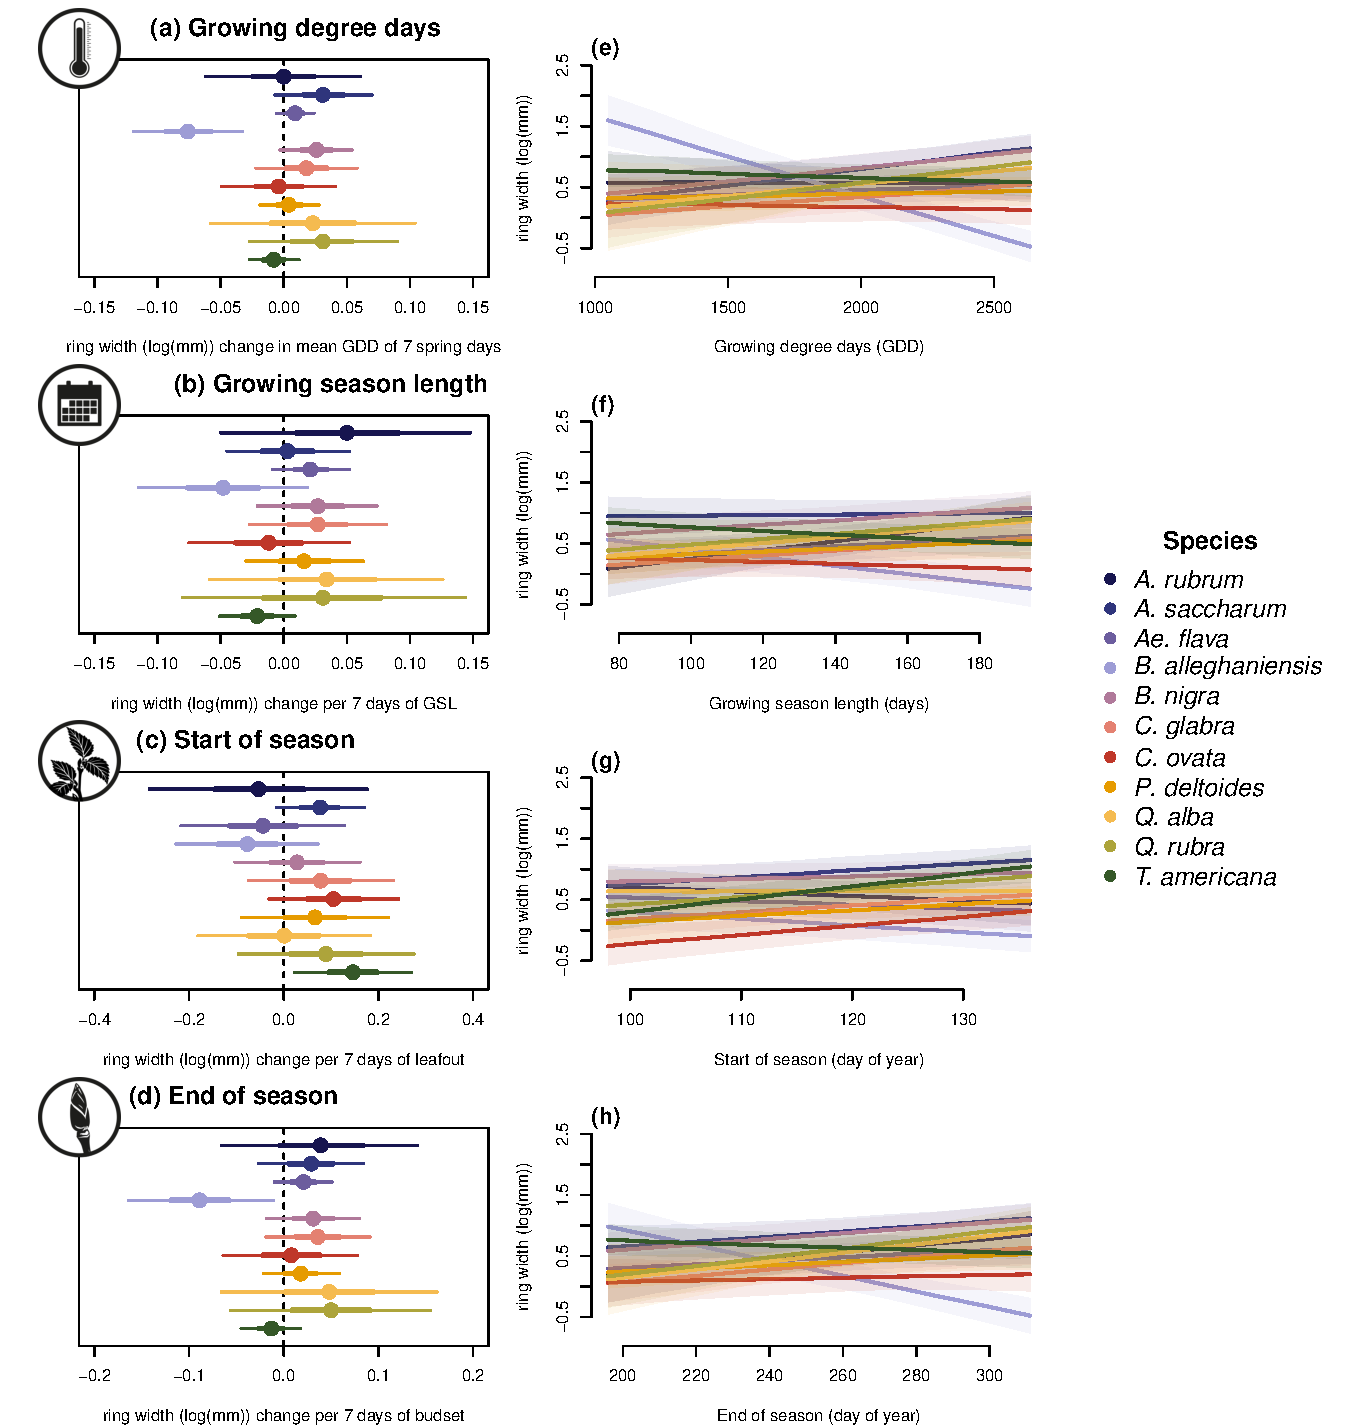
\includegraphics[width=0.8\textwidth]{../../analyses/figures/growthModelsMain/TSmuALLbsppWlines.pdf}
\caption{Estimates of ring width change (log(mm)) as a function of four different phenological predictors: growing degree days of the growing season (mean daily temperature above 5\degree C); growing season length; start of season; end of season across 11 species: (Red maple (\textit{Acer rubrum}), Sugar maple (\textit{Acer saccharum}), Yellow buckeye (\textit{Aesculus flava}), Yellow birch (\textit{Betula alleghaniensis}), River birch (\textit{Betula nigra}), Pignut hickory (\textit{Carya glabra}), Shagbark hickory (\textit{Carya ovata}), Eastern cottonwood (\textit{Populus deltoides}), White oak (\textit{Quercus alba}), Northern red oak (\textit{Quercus rubra}) and American basswood (\textit{Tilia americana})); species colors are the same across the panels). In the legend, the growth speed of each species is depicted as slow (S), moderate (M) and fast (F) and ring-porous (R) and diffuse-porous (D) correspond to their wood anatomy (Table \ref{tab:tsCount}). Panels on the left (a to d) represent the mean model slope estimates for each species (dots) with 50\% and 90\% uncertainty intervals (thicker and thinner lines, respectively), for each predictor, which we represent through ring width change in mm on the log scale per adjusted predictor (see `Data analyses' section in Methods for more details on predictor adjustment). See Table \ref{tab:ts_slope_table} for parameter estimates. Panels on the right (e to h) show the ring width response curves as a function of each predictor, with the lines depicting the mean response at each predictor value, and the shaded area, the 50\% uncertainty intervals. These models do not include an effect of the previous year GDD (see Figure \ref{fig:tsPrvsYr} for these estimates).}
\label{fig:tsmuplotbspp}
\end{figure}

% Figure mu previous year and current year
\begin{figure}[!ht]
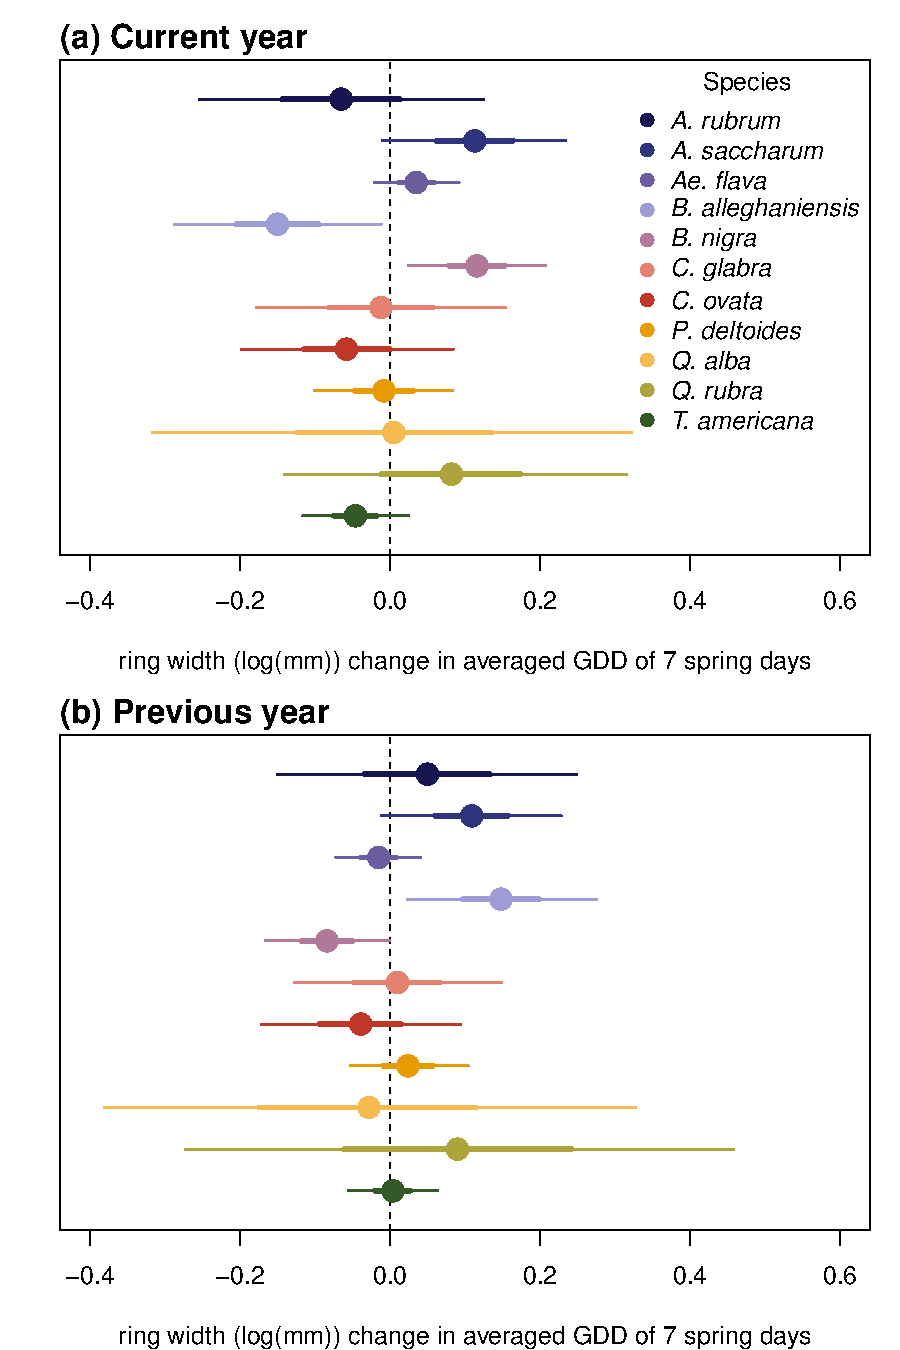
\includegraphics[width=0.6\textwidth]{../../analyses/figures/growthPreviousYearModel/bsppCurrentVSpreviousYR.pdf}
\caption{Model slope estimates representing ring width change (log(mm)) as a function of the current year growing degree days (GDD; a) and the previous year GDD (b) from a model considering both effects. GDD represent the accumulated growing degree days (mean daily temperature above 5\degree C)) between leafout and leaf colouring and the models estimates shows ring width change (log(mm)) per scaled GDD (see `Data analyses' section in Methods). The dots represent the mean of each species and the lines, the 50\% and 90\% uncertainty intervals (UI).}
\label{fig:tsPrvsYr}
\end{figure}

% latex table generated in R 4.5.1 by xtable 1.8-4 package
% Thu Jul 16 17:06:30 2026
\begin{table}[ht]
\centering
\caption{Species studied here grouped by growth speed and wood anatomy. We collected the growth speed information for each species from \cite{burns_silvics_1990}. We sampled a total of 49 individual trees} 
\label{tab:tsCount}
\begin{tabular}{p{7cm}p{5cm}p{3cm}r}
  \hline
Common Name (Latin binomial) & Growth speed & Wood Anatomy & $n$ \\
\hline
 \hline
 \textit{Acer rubrum} (Red maple) & Moderate & Diffuse-porous &   4 \\ 
  \textit{Acer saccharum} (Sugar maple) & Slow & Diffuse-porous &   5 \\ 
  \textit{Aesculus flava} (Yellow buckeye) & Moderate & Diffuse-porous &   5 \\ 
  \textit{Betula alleghaniensis} (Yellow birch) & Moderate & Diffuse-porous &   4 \\ 
  \textit{Betula nigra} (River birch) & Fast & Diffuse-porous &   4 \\ 
  \textit{Carya glabra} (Pignut hickory) & Slow & Ring-porous &   4 \\ 
  \textit{Carya ovata} (Shagbark hickory) & Moderate & Ring-porous &   5 \\ 
  \textit{Populus deltoides} (Eastern cottonwood) & Fast & Diffuse-porous &   4 \\ 
  \textit{Quercus alba} (White oak) & Slow & Ring-porous &   5 \\ 
  \textit{Quercus rubra} (Northern red oak) & Moderate & Ring-porous &   4 \\ 
  \textit{Tilia americana} (American basswood) & Fast & Diffuse-porous &   5 \\ 
   \hline
\end{tabular}
\end{table}


% <><><><><><><><><><><><><><><><><><><><><><><><><><><><><><><><><><><><><><><>
% DISCUSSION
% <><><><><><><><><><><><><><><><><><><><><><><><><><><><><><><><><><><><><><><>
\clearpage
\section{Discussion}
In this study, we used 49 trees of 11 species to understand if mature trees grew more with longer growing seasons. To do this, we used annual growth measured from tree rings and leaf phenology to estimate the SOS and EOS. Our findings reveal that warmer and longer growing seasons did not increase growth for any species and decreased growth for one. We also found that the previous year thermal conditions shifted growth trends for two species. 

Our findings support recent results that trees do not grow more with longer growing seasons. Some studies that have failed to find a connection between growth and growing season length did not consider species differences \citep[e.g.,][]{cabon_water_2020}, but others have looked specifically across species. The most comparable study \citep[with eight species in common to our dataset;][]{dow_warm_2022} was conducted geographically close to ours and found similar results: despite warmer and earlier springs, trees did not grow more. Our results complement these findings as we used leaf phenology and have EOS and SOS, while the previous study only had SOS for growth phenology and not leaf phenology. In addition, \cite{cufar_variations_2015} had substantially more years (five decades) and found analogous results to ours, but only for one European species, \textit{Fagus Sylvatica}. Taken together, these results support the idea that longer growing seasons may not increase temperate tree growth, a least for mature trees. 

We previously showed (see Chapter 1) that our studied juvenile trees grew more with longer and warmer growing seasons, contrasting with the response we found here with mature trees. Interestingly, these diverging responses corroborate the assumption that younger trees are usually more responsive to changing conditions compared to mature trees \citep{wolkovich_why_2025}. This common garden study looked at a few number of species with rather homogeneous life-history strategies, but our study on mature trees in the arboretum comprised more distant species spanning a wider range of life-history strategies. These fast-growing juvenile trees all grew more with warmer seasons. However, our mature trees did not show a strong signal of life-history strategies in their growth response to growing season conditions, with even the fastest growing species (i.e. {\Bnig}, {\Pdel} and {\Tame}) barely showing responding to warmer seasons.

\subsection{Life-history influence on growth trends}
While our species share an array of growth strategies (see Table \ref{tab:tsCount}), we did not find a consistent growth trend across them. Only {\Ball}, which has a moderately fast-growth, responded to the thermal season and its decrease in growth suggests it may be negatively impacted by warmer seasons. {\Ball} also grew less with a later EOS, which is a period characterized by fast GDD accumulation. The fact that {\Ball} appears to be negatively impacted by warmer seasons suggests that this species could face declines at its southernmost range where its growth may not keep up with warmer and longer seasons \citep{doak_demographic_2010,aitken_adaptation_2008}. In contrast to {\Ball}, its congeneric species, {\Bnig}, increased in growth with warmer seasons (though only when the previous year conditions were included). {\Bnig} is faster growing than {\Ball}, which may explain its response, though we did not find any consistent response across the other fast growing species. Indeed, the fast-growing {\Tame} \citep[Table \ref{tab:tsCount};][]{burns_silvics_1990} grew less with an earlier SOS---when the days are short and cool. This is contrast with our expectation of species with this rapid life-history strategy which should provide them an edge by starting to grow earlier in the season \citep{loughnan_budburst_2025}. The other eight species had different life-history strategies (fast: {\Pdel}; moderate: {\Arub}, {\Afla}, {\Cova}, {\Qrub}; slow: {\Asac}, {\Cgla}, {\Qalb}; Table \ref{tab:tsCount}), and despite this diversity in growth speed, none changed their growth with longer seasons. Ultimately, these findings suggest a weak signal of life-history strategies in growth responses to longer and warmer growing seasons.

We also found no clear trends with ring porosity. {\Ball} and {\Bnig}, which showed the contrasting responses described above were both diffuse-porous and the five other diffuse-porous species ({\Afla}, {\Arub}, {\Asac}, {\Pdel} and {\Tame}) did not increase growth with longer or warmer seasons. We had only four ring-porous species ({\Cgla}, {\Cova}, {\Qalb} and {\Qrub}), which responded similarly to the diffuse-porous species. While this is a small sample, it supports recent work \citep[e.g.,][]{grover_growth_2023} suggesting ring porosity may not be as useful a predictor for growth as previously suggested \citep{wang_relation_1992}. While wood porosity imposes inherent physiological differences across species, this dichotomous classification may over-simplify the reality of the complex dynamic of tree growth. In fact, a gradient of life history strategies may exist within each wood porosity type where both fast and slow growing species can share the same wood porosity, though this is poorly documented \citep{taneda_casestudy_2008}. This emphasizes the need to better classify growth traits and related carbon allocation with wood porosity. 

\subsection{Growth response blurred by carbon allocation to storage}
Shifts in our findings when including previous year thermal season suggest including carbon allocation strategy may be important to understanding how longer growing seasons affect growth. The growth response of two \textit{Betula} species shifted when we included the previous year thermal season as a driver. These two congeneric and diffuse-porous species ({\Ball} and {\Bnig}) had diametrically opposed responses, however. {\Ball} growth decreased with the current year thermal conditions, but increased with a warmer previous year, possibly revealing a carbon allocation strategy that prioritizes carbon storage above short-term growth. This is in contrast with the expectation that diffuse-porous species will tend to allocate less carbon to storage and more to growth \citep{barbaroux_contrasting_2002,muhr_how_2016}. In contrast, {\Bnig} increased in growth during the current year---only when the previous year conditions were included---supporting the expectation that diffuse-porous species prioritize rapid investment in growth with less allocation to storage. These opposite responses of two closely related species, highlight the importance of considering more than the current year in tree growth and growing season length models.

Also, considering conditions beyond the current year when studying mature tree growth could help elucidate tree growth dynamics. Even if some species do not have complex storage dynamics, they still allocate carbon to reproduction that may blur their growth responses. Our findings reveal a weak response of the growing season length and conditions on growth across 11 species, corroborating previous findings on mature trees \citep{cufar_treering_2008,delpierre_temperate_2016,silvestro_longer_2023}. If carbon allocation to storage and reproduction, life-history strategies and differences in wood anatomy blur growth responses as we suggest, further studies leveraging a larger sample size should be specifically designed to tease these factors apart.

%<><><><><><><><><><><><><><><><><><><><><><><><><><><><><><><><><><><><><><><><>
% REFERENCES %
%<><><><><><><><><><><><><><><><><><><><><><><><><><><><><><><><><><><><><><><><>
\bibliography{ExportedItems}
\bibliographystyle{ecolett} 

% <><><><><><><><><><><><><><><><><><><><><><><><><><><><><><><><><><><><><><><>
% SUPPLEMENT
% <><><><><><><><><><><><><><><><><><><><><><><><><><><><><><><><><><><><><><><>
\clearpage

\section{Supplemental material}

\setcounter{table}{0}
\renewcommand{\thetable}{S\arabic{table}}
\setcounter{figure}{0}
\renewcommand{\thefigure}{S\arabic{figure}}

% Rw per year for allometry
\begin{figure}[!ht]

\includegraphics[width=0.6\textwidth]{/Users/christophe_rouleau-desrochers/github/coringTreespotters/analyses/figures/empiricalData/rwXyearRestricted.pdf}
\caption{We randomly sampled 20 trees from our dataset and represent the ring width as a function of year to represent the allometry patterns across all years we had phenology data for.}
\label{fig:allom}
\end{figure}

%-------------------------------------------------------------------------------
% Supplemental Results
%-------------------------------------------------------------------------------

% latex table generated in R 4.5.1 by xtable 1.8-4 package
% Thu Jul 16 17:06:30 2026
\begin{table}[ht]
\centering
\caption{Species level slope parameters which represent ring width change (log(mm)), per scaled predictor (see `Data analyses' section in Methods for more details on predictor scaling). We report estimates as mean and 90\% uncertainty intervals (in square brackets) across our four different predictors (GDD: growing degree days, GSL: growing season length, SOS: start of season and EOS: end of season). Table \ref{tab:tab_all} reports all the models parameters.} 
\label{tab:ts_slope_table}
\begin{tabular}{lllll}
  \hline
Species & GDD & GSL & SOS & EOS \\ 
  \hline
\textit{A. rubrum} & 0.00 [-0.06, 0.06] & 0.05 [-0.05, 0.15] & -0.05 [-0.28, 0.18] & 0.04 [-0.07, 0.14] \\ 
  \textit{A. saccharum} & 0.03 [-0.01, 0.07] & 0.00 [-0.04, 0.05] & 0.08 [-0.02, 0.17] & 0.03 [-0.03, 0.08] \\ 
  \textit{Ae. flava} & 0.01 [-0.01, 0.02] & 0.02 [-0.01, 0.05] & -0.04 [-0.22, 0.13] & 0.02 [-0.01, 0.05] \\ 
  \textit{B. alleghaniensis} & -0.08 [-0.12, -0.03] & -0.05 [-0.12, 0.02] & -0.08 [-0.23, 0.07] & -0.09 [-0.16, -0.01] \\ 
  \textit{B. nigra} & 0.03 [-0.00, 0.05] & 0.03 [-0.02, 0.07] & 0.03 [-0.10, 0.16] & 0.03 [-0.02, 0.08] \\ 
  \textit{C. glabra} & 0.02 [-0.02, 0.06] & 0.03 [-0.03, 0.08] & 0.08 [-0.07, 0.23] & 0.04 [-0.02, 0.09] \\ 
  \textit{C. ovata} & -0.00 [-0.05, 0.04] & -0.01 [-0.07, 0.05] & 0.10 [-0.03, 0.24] & 0.01 [-0.06, 0.08] \\ 
  \textit{P. deltoides} & 0.00 [-0.02, 0.03] & 0.02 [-0.03, 0.06] & 0.07 [-0.09, 0.22] & 0.02 [-0.02, 0.06] \\ 
  \textit{Q. alba} & 0.02 [-0.06, 0.10] & 0.03 [-0.06, 0.13] & 0.00 [-0.18, 0.18] & 0.05 [-0.07, 0.16] \\ 
  \textit{Q. rubra} & 0.03 [-0.03, 0.09] & 0.03 [-0.08, 0.14] & 0.09 [-0.10, 0.28] & 0.05 [-0.06, 0.15] \\ 
  \textit{T. americana} & -0.01 [-0.03, 0.01] & -0.02 [-0.05, 0.01] & 0.15 [0.02, 0.27] & -0.01 [-0.04, 0.02] \\ 
   \hline
\end{tabular}
\end{table}



% latex table generated in R 4.5.1 by xtable 1.8-4 package
% Thu Jul 16 17:06:30 2026
\begin{table}[ht]
\centering
\caption{Summary output of each parameter from our four predictors, using ring width (log(mm)) as the response variable (See equation \ref{eq:mainMdl}). We report estimates as mean and 90\% uncertainty intervals (in square brackets) across our four different predictors (GDD: growing degree days, GSL: growing season length, SOS: start of season and EOS: end of season). See `Data analyses' section in Methods for more details.} 
\label{tab:tab_all}
\begin{tabular}{lllll}
  \hline
Parameter & GDD & GSL & SOS & EOS \\ 
  \hline
$\alpha$ & 0.61 [-2.08, 3.25] & 0.49 [-2.09, 3.03] & 0.24 [-2.39, 2.94] & 0.23 [-2.48, 2.98] \\ 
  $\sigma_{\alpha_{tree}}$ & 0.55 [0.45, 0.67] & 0.55 [0.45, 0.68] & 0.54 [0.44, 0.66] & 0.55 [0.45, 0.67] \\ 
  $\sigma_{y}$ & 0.31 [0.29, 0.34] & 0.32 [0.29, 0.34] & 0.32 [0.29, 0.34] & 0.32 [0.29, 0.34] \\ 
  $\beta_{species_{A. rubrum}}$ & 0.00 [-0.06, 0.06] & 0.05 [-0.05, 0.15] & -0.05 [-0.28, 0.18] & 0.04 [-0.07, 0.14] \\ 
  $\beta_{species_{A. saccharum}}$ & 0.03 [-0.01, 0.07] & 0.00 [-0.04, 0.05] & 0.08 [-0.02, 0.17] & 0.03 [-0.03, 0.08] \\ 
  $\beta_{species_{Ae. flava}}$ & 0.01 [-0.01, 0.02] & 0.02 [-0.01, 0.05] & -0.04 [-0.22, 0.13] & 0.02 [-0.01, 0.05] \\ 
  $\beta_{species_{B. alleghaniensis}}$ & -0.08 [-0.12, -0.03] & -0.05 [-0.12, 0.02] & -0.08 [-0.23, 0.07] & -0.09 [-0.16, -0.01] \\ 
  $\beta_{species_{B. nigra}}$ & 0.03 [-0.00, 0.05] & 0.03 [-0.02, 0.07] & 0.03 [-0.10, 0.16] & 0.03 [-0.02, 0.08] \\ 
  $\beta_{species_{C. glabra}}$ & 0.02 [-0.02, 0.06] & 0.03 [-0.03, 0.08] & 0.08 [-0.07, 0.23] & 0.04 [-0.02, 0.09] \\ 
  $\beta_{species_{C. ovata}}$ & -0.00 [-0.05, 0.04] & -0.01 [-0.07, 0.05] & 0.10 [-0.03, 0.24] & 0.01 [-0.06, 0.08] \\ 
  $\beta_{species_{P. deltoides}}$ & 0.00 [-0.02, 0.03] & 0.02 [-0.03, 0.06] & 0.07 [-0.09, 0.22] & 0.02 [-0.02, 0.06] \\ 
  $\beta_{species_{Q. alba}}$ & 0.02 [-0.06, 0.10] & 0.03 [-0.06, 0.13] & 0.00 [-0.18, 0.18] & 0.05 [-0.07, 0.16] \\ 
  $\beta_{species_{Q. rubra}}$ & 0.03 [-0.03, 0.09] & 0.03 [-0.08, 0.14] & 0.09 [-0.10, 0.28] & 0.05 [-0.06, 0.15] \\ 
  $\beta_{species_{T. americana}}$ & -0.01 [-0.03, 0.01] & -0.02 [-0.05, 0.01] & 0.15 [0.02, 0.27] & -0.01 [-0.04, 0.02] \\ 
  $\alpha_{year_{2016}}$ & -0.05 [-3.40, 3.35] & -0.95 [-4.12, 2.17] & 1.23 [-3.23, 5.60] & -1.08 [-5.62, 3.44] \\ 
  $\alpha_{year_{2017}}$ & -0.90 [-3.86, 2.10] & 0.43 [-2.34, 3.17] & -0.57 [-3.59, 2.35] & -0.37 [-3.79, 3.02] \\ 
  $\alpha_{year_{2018}}$ & -0.49 [-3.20, 2.19] & -0.46 [-3.09, 2.14] & 0.93 [-2.69, 4.47] & -0.49 [-3.33, 2.38] \\ 
  $\alpha_{year_{2019}}$ & 2.32 [-0.68, 5.34] & 0.61 [-2.29, 3.46] & 1.17 [-2.34, 4.58] & 3.25 [-0.47, 6.96] \\ 
  $\alpha_{year_{2020}}$ & -0.68 [-3.54, 2.12] & -0.13 [-2.82, 2.58] & 0.17 [-3.18, 3.40] & -0.50 [-3.65, 2.67] \\ 
  $\alpha_{year_{2021}}$ & -0.89 [-3.89, 2.06] & -0.64 [-3.44, 2.12] & -1.17 [-4.65, 2.33] & -1.16 [-4.46, 2.12] \\ 
  $\alpha_{year_{2022}}$ & -0.32 [-3.35, 2.74] & -0.07 [-2.88, 2.73] & -1.96 [-5.42, 1.40] & -0.35 [-4.01, 3.29] \\ 
  $\alpha_{year_{2023}}$ & -0.38 [-3.14, 2.40] & -0.39 [-3.09, 2.26] & -1.04 [-4.60, 2.52] & -0.49 [-3.54, 2.50] \\ 
  $\alpha_{year_{2024}}$ & -0.85 [-4.70, 3.03] & -0.56 [-3.66, 2.52] & 0.40 [-3.47, 4.32] & -1.44 [-6.32, 3.48] \\ 
  $\alpha_{species_{A. rubrum}}$ & -1.09 [-4.47, 2.23] & -0.43 [-3.80, 2.96] & -1.08 [-4.98, 2.91] & -1.44 [-6.04, 3.22] \\ 
  $\alpha_{species_{A. saccharum}}$ & 0.30 [-2.41, 3.02] & 0.59 [-1.98, 3.18] & -2.02 [-5.24, 1.14] & 0.92 [-1.93, 3.81] \\ 
  $\alpha_{species_{Ae. flava}}$ & -0.21 [-0.77, 0.34] & -0.22 [-0.76, 0.35] & -0.25 [-0.80, 0.31] & -0.25 [-0.81, 0.29] \\ 
  $\alpha_{species_{B. alleghaniensis}}$ & -0.03 [-0.58, 0.52] & -0.06 [-0.59, 0.52] & 0.00 [-0.54, 0.56] & -0.07 [-0.63, 0.48] \\ 
  $\alpha_{species_{B. nigra}}$ & 0.04 [-0.52, 0.59] & 0.02 [-0.52, 0.59] & -0.00 [-0.55, 0.56] & 0.01 [-0.54, 0.56] \\ 
  $\alpha_{species_{C. glabra}}$ & 0.09 [-0.46, 0.64] & 0.06 [-0.48, 0.63] & 0.07 [-0.47, 0.64] & 0.06 [-0.50, 0.62] \\ 
  $\alpha_{species_{C. ovata}}$ & -0.06 [-0.60, 0.49] & -0.07 [-0.61, 0.50] & -0.12 [-0.66, 0.45] & -0.07 [-0.63, 0.47] \\ 
  $\alpha_{species_{P. deltoides}}$ & 0.00 [-0.55, 0.56] & -0.00 [-0.55, 0.57] & 0.01 [-0.54, 0.58] & -0.01 [-0.58, 0.54] \\ 
  $\alpha_{species_{Q. alba}}$ & -0.05 [-0.61, 0.50] & -0.07 [-0.63, 0.50] & -0.07 [-0.63, 0.49] & -0.08 [-0.65, 0.48] \\ 
  $\alpha_{species_{Q. rubra}}$ & 0.20 [-0.36, 0.76] & 0.18 [-0.38, 0.75] & 0.20 [-0.35, 0.78] & 0.17 [-0.40, 0.72] \\ 
  $\alpha_{species_{T. americana}}$ & 0.08 [-0.47, 0.64] & 0.07 [-0.47, 0.66] & 0.07 [-0.48, 0.64] & 0.08 [-0.49, 0.64] \\ 
   \hline
\end{tabular}
\end{table}


% latex table generated in R 4.5.1 by xtable 1.8-4 package
% Thu Jul 16 17:06:30 2026
\begin{table}[ht]
\centering
\caption{Summary output of each parameter from the previous year model (Equation \ref{eq:prvsYrMdl}) using ring width (log(mm)) as the response variable. We report estimates as mean and 90\% uncertainty intervals (in square brackets). see `Data analyses' section in Methods for more details} 
\label{tab:tab_PrvsYr}
\begin{tabular}{ll}
  \hline
Parameter & Estimate \\ 
  \hline
$\alpha$ & 0.20 [-1.10, 1.48] \\ 
  $\sigma_{\alpha_{tree}}$ & 0.58 [0.47, 0.72] \\ 
  $\sigma_{y}$ & 0.29 [0.26, 0.32] \\ 
  $\beta_{\text{species}_{A. rubrum}}^{\text{current}}$ & -0.07 [-0.25, 0.12] \\ 
  $\beta_{\text{species}_{A. saccharum}}^{\text{current}}$ & 0.11 [-0.01, 0.23] \\ 
  $\beta_{\text{species}_{Ae. flava}}^{\text{current}}$ & 0.04 [-0.02, 0.09] \\ 
  $\beta_{\text{species}_{B. alleghaniensis}}^{\text{current}}$ & -0.15 [-0.29, -0.01] \\ 
  $\beta_{\text{species}_{B. nigra}}^{\text{current}}$ & 0.12 [0.03, 0.21] \\ 
  $\beta_{\text{species}_{C. glabra}}^{\text{current}}$ & -0.01 [-0.18, 0.15] \\ 
  $\beta_{\text{species}_{C. ovata}}^{\text{current}}$ & -0.06 [-0.20, 0.08] \\ 
  $\beta_{\text{species}_{P. deltoides}}^{\text{current}}$ & -0.01 [-0.10, 0.08] \\ 
  $\beta_{\text{species}_{Q. alba}}^{\text{current}}$ & 0.01 [-0.32, 0.32] \\ 
  $\beta_{\text{species}_{Q. rubra}}^{\text{current}}$ & 0.08 [-0.14, 0.32] \\ 
  $\beta_{\text{species}_{T. americana}}^{\text{current}}$ & -0.05 [-0.12, 0.03] \\ 
  $\beta_{\text{species}_{A. rubrum}}^{\text{previous}}$ & 0.05 [-0.15, 0.25] \\ 
  $\beta_{\text{species}_{A. saccharum}}^{\text{previous}}$ & 0.11 [-0.01, 0.23] \\ 
  $\beta_{\text{species}_{Ae. flava}}^{\text{previous}}$ & -0.01 [-0.07, 0.04] \\ 
  $\beta_{\text{species}_{B. alleghaniensis}}^{\text{previous}}$ & 0.15 [0.02, 0.28] \\ 
  $\beta_{\text{species}_{B. nigra}}^{\text{previous}}$ & -0.08 [-0.17, -0.00] \\ 
  $\beta_{\text{species}_{C. glabra}}^{\text{previous}}$ & 0.01 [-0.13, 0.15] \\ 
  $\beta_{\text{species}_{C. ovata}}^{\text{previous}}$ & -0.04 [-0.17, 0.09] \\ 
  $\beta_{\text{species}_{P. deltoides}}^{\text{previous}}$ & 0.02 [-0.05, 0.10] \\ 
  $\beta_{\text{species}_{Q. alba}}^{\text{previous}}$ & -0.03 [-0.38, 0.33] \\ 
  $\beta_{\text{species}_{Q. rubra}}^{\text{previous}}$ & 0.09 [-0.27, 0.46] \\ 
  $\beta_{\text{species}_{T. americana}}^{\text{previous}}$ & 0.00 [-0.06, 0.06] \\ 
  $\alpha_{\text{year}_{2016}}$ & 0.44 [-3.10, 3.90] \\ 
  $\alpha_{\text{year}_{2017}}$ & -2.20 [-4.79, 0.36] \\ 
  $\alpha_{\text{year}_{2018}}$ & 0.04 [-1.53, 1.59] \\ 
  $\alpha_{\text{year}_{2019}}$ & -0.06 [-2.61, 2.44] \\ 
  $\alpha_{\text{year}_{2020}}$ & 0.30 [-1.39, 1.99] \\ 
  $\alpha_{\text{year}_{2021}}$ & 0.18 [-1.77, 2.13] \\ 
  $\alpha_{\text{year}_{2022}}$ & 1.16 [-1.18, 3.47] \\ 
  $\alpha_{\text{year}_{2023}}$ & -0.01 [-1.92, 1.90] \\ 
  $\alpha_{\text{year}_{2024}}$ & 0.97 [-5.55, 7.68] \\ 
  $\alpha_{\text{species}_{A. rubrum}}$ & -1.73 [-8.12, 4.60] \\ 
  $\alpha_{\text{species}_{A. saccharum}}$ & 0.93 [-0.65, 2.50] \\ 
  $\alpha_{\text{species}_{Ae. flava}}$ & 0.07 [-0.48, 0.62] \\ 
  $\alpha_{\text{species}_{B. alleghaniensis}}$ & 0.06 [-0.50, 0.61] \\ 
  $\alpha_{\text{species}_{B. nigra}}$ & -0.30 [-1.02, 0.42] \\ 
  $\alpha_{\text{species}_{C. glabra}}$ & -0.04 [-0.58, 0.53] \\ 
  $\alpha_{\text{species}_{C. ovata}}$ & 0.00 [-0.55, 0.56] \\ 
  $\alpha_{\text{species}_{P. deltoides}}$ & -0.00 [-0.56, 0.56] \\ 
  $\alpha_{\text{species}_{Q. alba}}$ & 0.17 [-0.40, 0.73] \\ 
  $\alpha_{\text{species}_{Q. rubra}}$ & 0.01 [-0.56, 0.58] \\ 
  $\alpha_{\text{species}_{T. americana}}$ & -0.05 [-0.60, 0.51] \\ 
   \hline
\end{tabular}
\end{table}


% latex table generated in R 4.5.1 by xtable 1.8-4 package
% Thu Jul 16 17:06:30 2026
\begin{table}[ht]
\centering
\caption{Summary output of each parameter from the model on the effect of SOS (days) on EOS (days; Equation \ref{eq:SOSonEOSMdl}). We report estimates as mean and 90\% uncertainty intervals (in square brackets). see `Data analyses' section in Methods for more details} 
\label{tab:tab_PrvsYr}
\begin{tabular}{ll}
  \hline
Parameter & Estimate \\ 
  \hline
$\alpha$ & 29.51 [23.54, 35.39] \\ 
  $\sigma_{\alpha_{treeid}}$ & 1.18 [0.83, 1.56] \\ 
  $\sigma_{y}$ & 2.06 [1.90, 2.23] \\ 
  $\beta_{\text{species}_{A. rubrum}}$ & 0.63 [-0.14, 1.42] \\ 
  $\beta_{\text{species}_{A. saccharum}}$ & 0.18 [-0.29, 0.66] \\ 
  $\beta_{\text{species}_{Ae. flava}}$ & 0.38 [-0.32, 1.08] \\ 
  $\beta_{\text{species}_{B. alleghaniensis}}$ & 0.50 [-0.15, 1.16] \\ 
  $\beta_{\text{species}_{B. nigra}}$ & 0.44 [-0.16, 1.06] \\ 
  $\beta_{\text{species}_{C. glabra}}$ & 0.48 [-0.17, 1.15] \\ 
  $\beta_{\text{species}_{C. ovata}}$ & 0.40 [-0.22, 1.01] \\ 
  $\beta_{\text{species}_{P. deltoides}}$ & 1.04 [0.39, 1.70] \\ 
  $\beta_{\text{species}_{Q. alba}}$ & 0.35 [-0.34, 1.04] \\ 
  $\beta_{\text{species}_{Q. rubra}}$ & 0.50 [-0.19, 1.22] \\ 
  $\beta_{\text{species}_{T. americana}}$ & 0.46 [-0.14, 1.05] \\ 
  $\alpha_{\text{year}_{2016}}$ & -2.26 [-15.00, 10.18] \\ 
  $\alpha_{\text{year}_{2017}}$ & 7.21 [-1.83, 16.23] \\ 
  $\alpha_{\text{year}_{2018}}$ & 0.36 [-10.75, 11.25] \\ 
  $\alpha_{\text{year}_{2019}}$ & -0.23 [-11.38, 10.91] \\ 
  $\alpha_{\text{year}_{2020}}$ & 0.27 [-10.43, 10.84] \\ 
  $\alpha_{\text{year}_{2021}}$ & -0.20 [-11.26, 10.69] \\ 
  $\alpha_{\text{year}_{2022}}$ & 1.92 [-9.19, 13.03] \\ 
  $\alpha_{\text{year}_{2023}}$ & -11.53 [-23.17, 0.25] \\ 
  $\alpha_{\text{year}_{2024}}$ & 3.61 [-8.48, 15.48] \\ 
  $\alpha_{\text{species}_{A. rubrum}}$ & 0.14 [-12.16, 12.19] \\ 
  $\alpha_{\text{species}_{A. saccharum}}$ & -0.27 [-10.42, 9.76] \\ 
  $\alpha_{\text{species}_{Ae. flava}}$ & 1.86 [-0.38, 4.14] \\ 
  $\alpha_{\text{species}_{B. alleghaniensis}}$ & 1.17 [-1.06, 3.41] \\ 
  $\alpha_{\text{species}_{B. nigra}}$ & 0.47 [-1.80, 2.72] \\ 
  $\alpha_{\text{species}_{C. glabra}}$ & -0.42 [-2.70, 1.80] \\ 
  $\alpha_{\text{species}_{C. ovata}}$ & -1.02 [-3.27, 1.27] \\ 
  $\alpha_{\text{species}_{P. deltoides}}$ & -0.23 [-2.54, 2.06] \\ 
  $\alpha_{\text{species}_{Q. alba}}$ & -0.87 [-3.21, 1.45] \\ 
  $\alpha_{\text{species}_{Q. rubra}}$ & -0.28 [-2.63, 2.06] \\ 
  $\alpha_{\text{species}_{T. americana}}$ & -1.50 [-3.85, 0.81] \\ 
   \hline
\end{tabular}
\end{table}


% Coringtreespotters year mu plot
\begin{figure}[!ht]
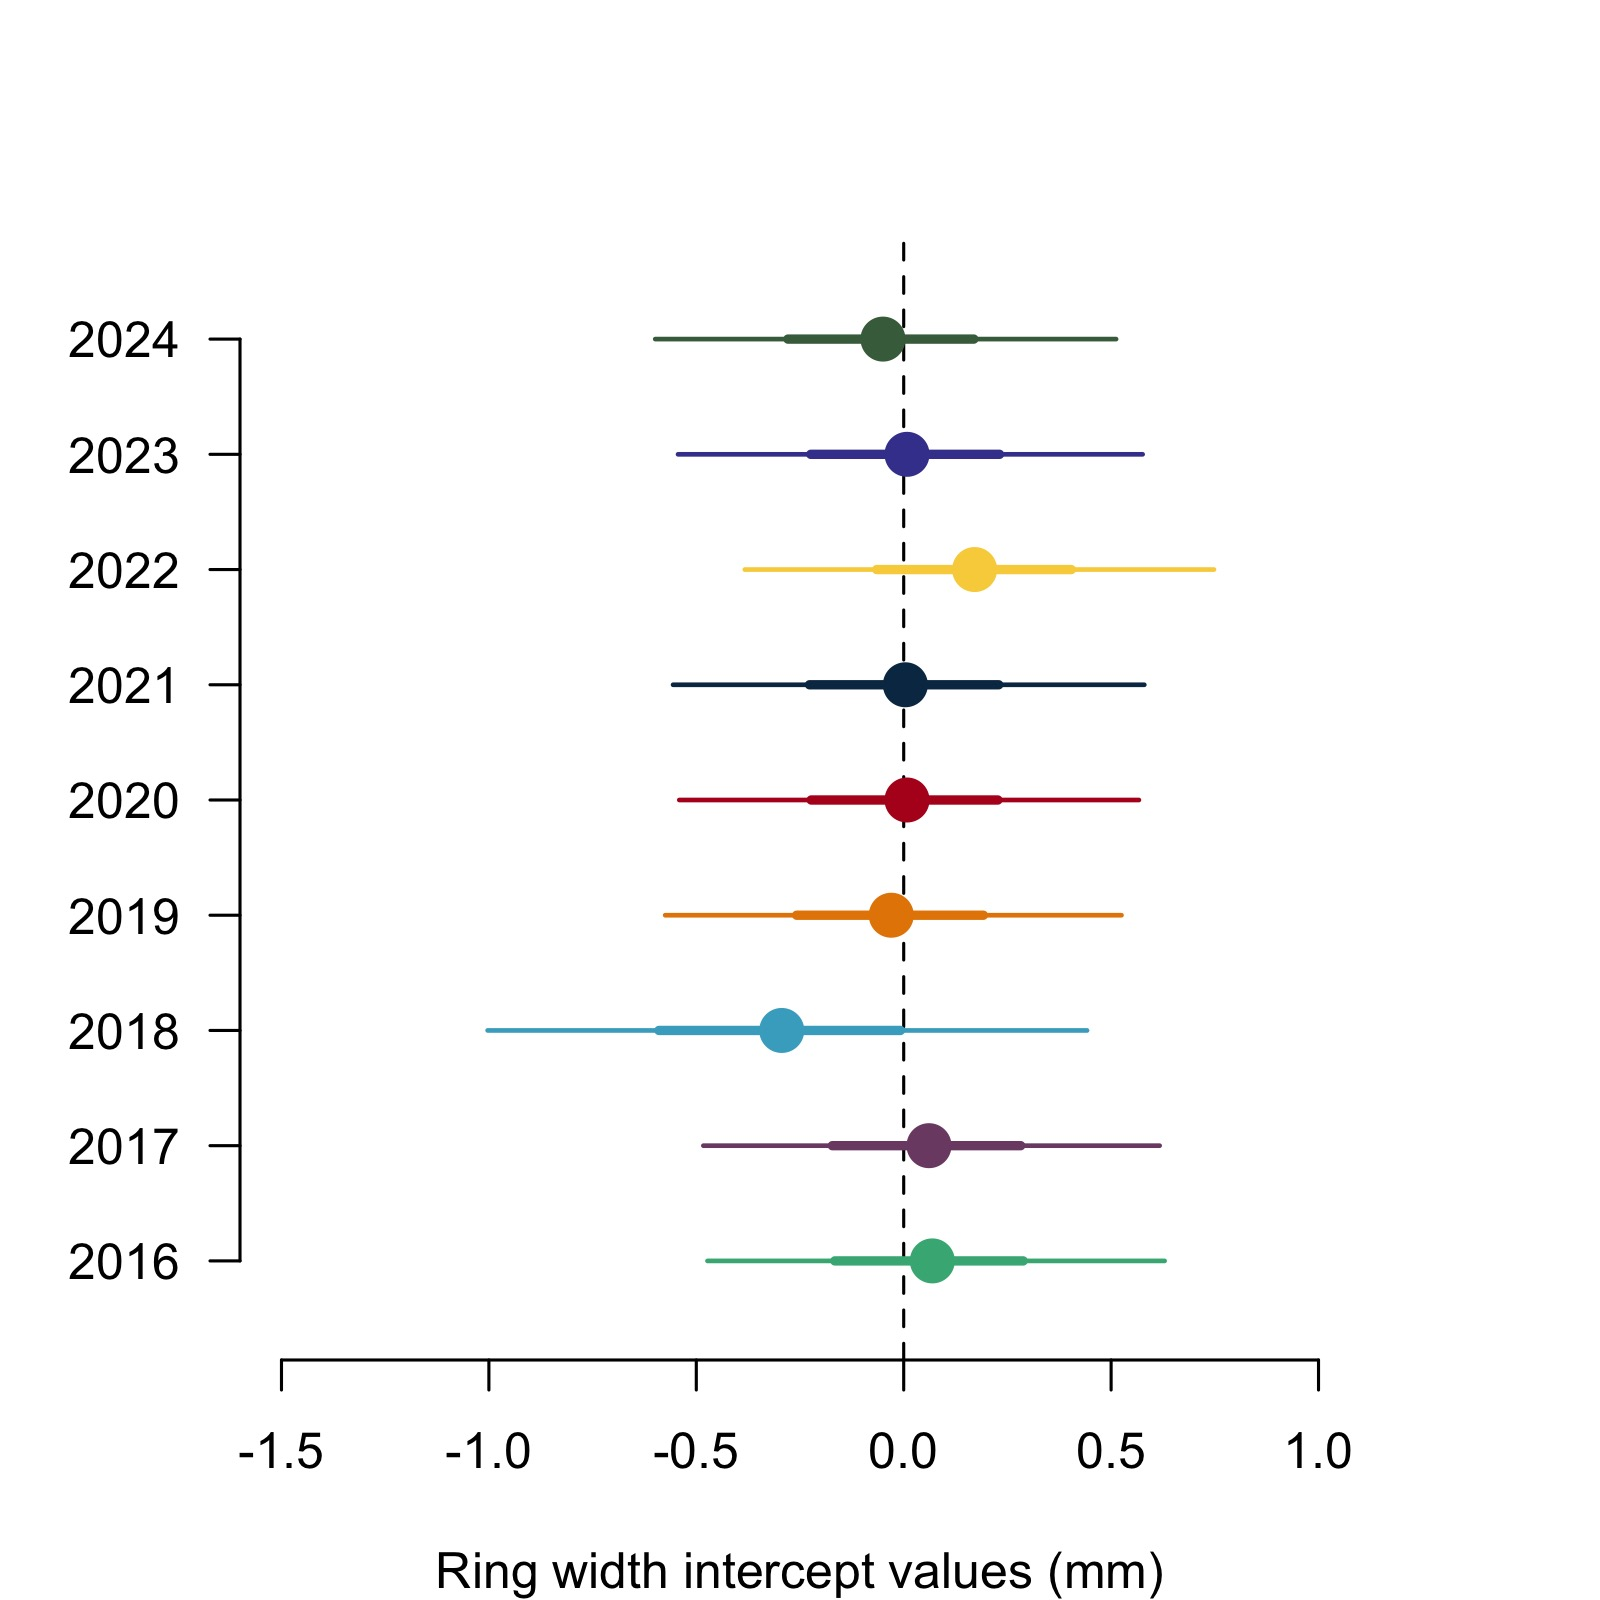
\includegraphics[width=0.5\textwidth]{../../analyses/figures/growthModelsMain/TSmuayear}
\caption{Ring width (log(mm)) deviations from the grand mean for each year using the GDD model (Table \ref{tab:tab_all}). The dots are the mean of the posterior distribution and the thick and thin lines, the 50 and 90\% UI.}
\label{fig:tsmuplotayear}
\end{figure}

% Coringtreespotters boxplot
\begin{figure}[!ht]
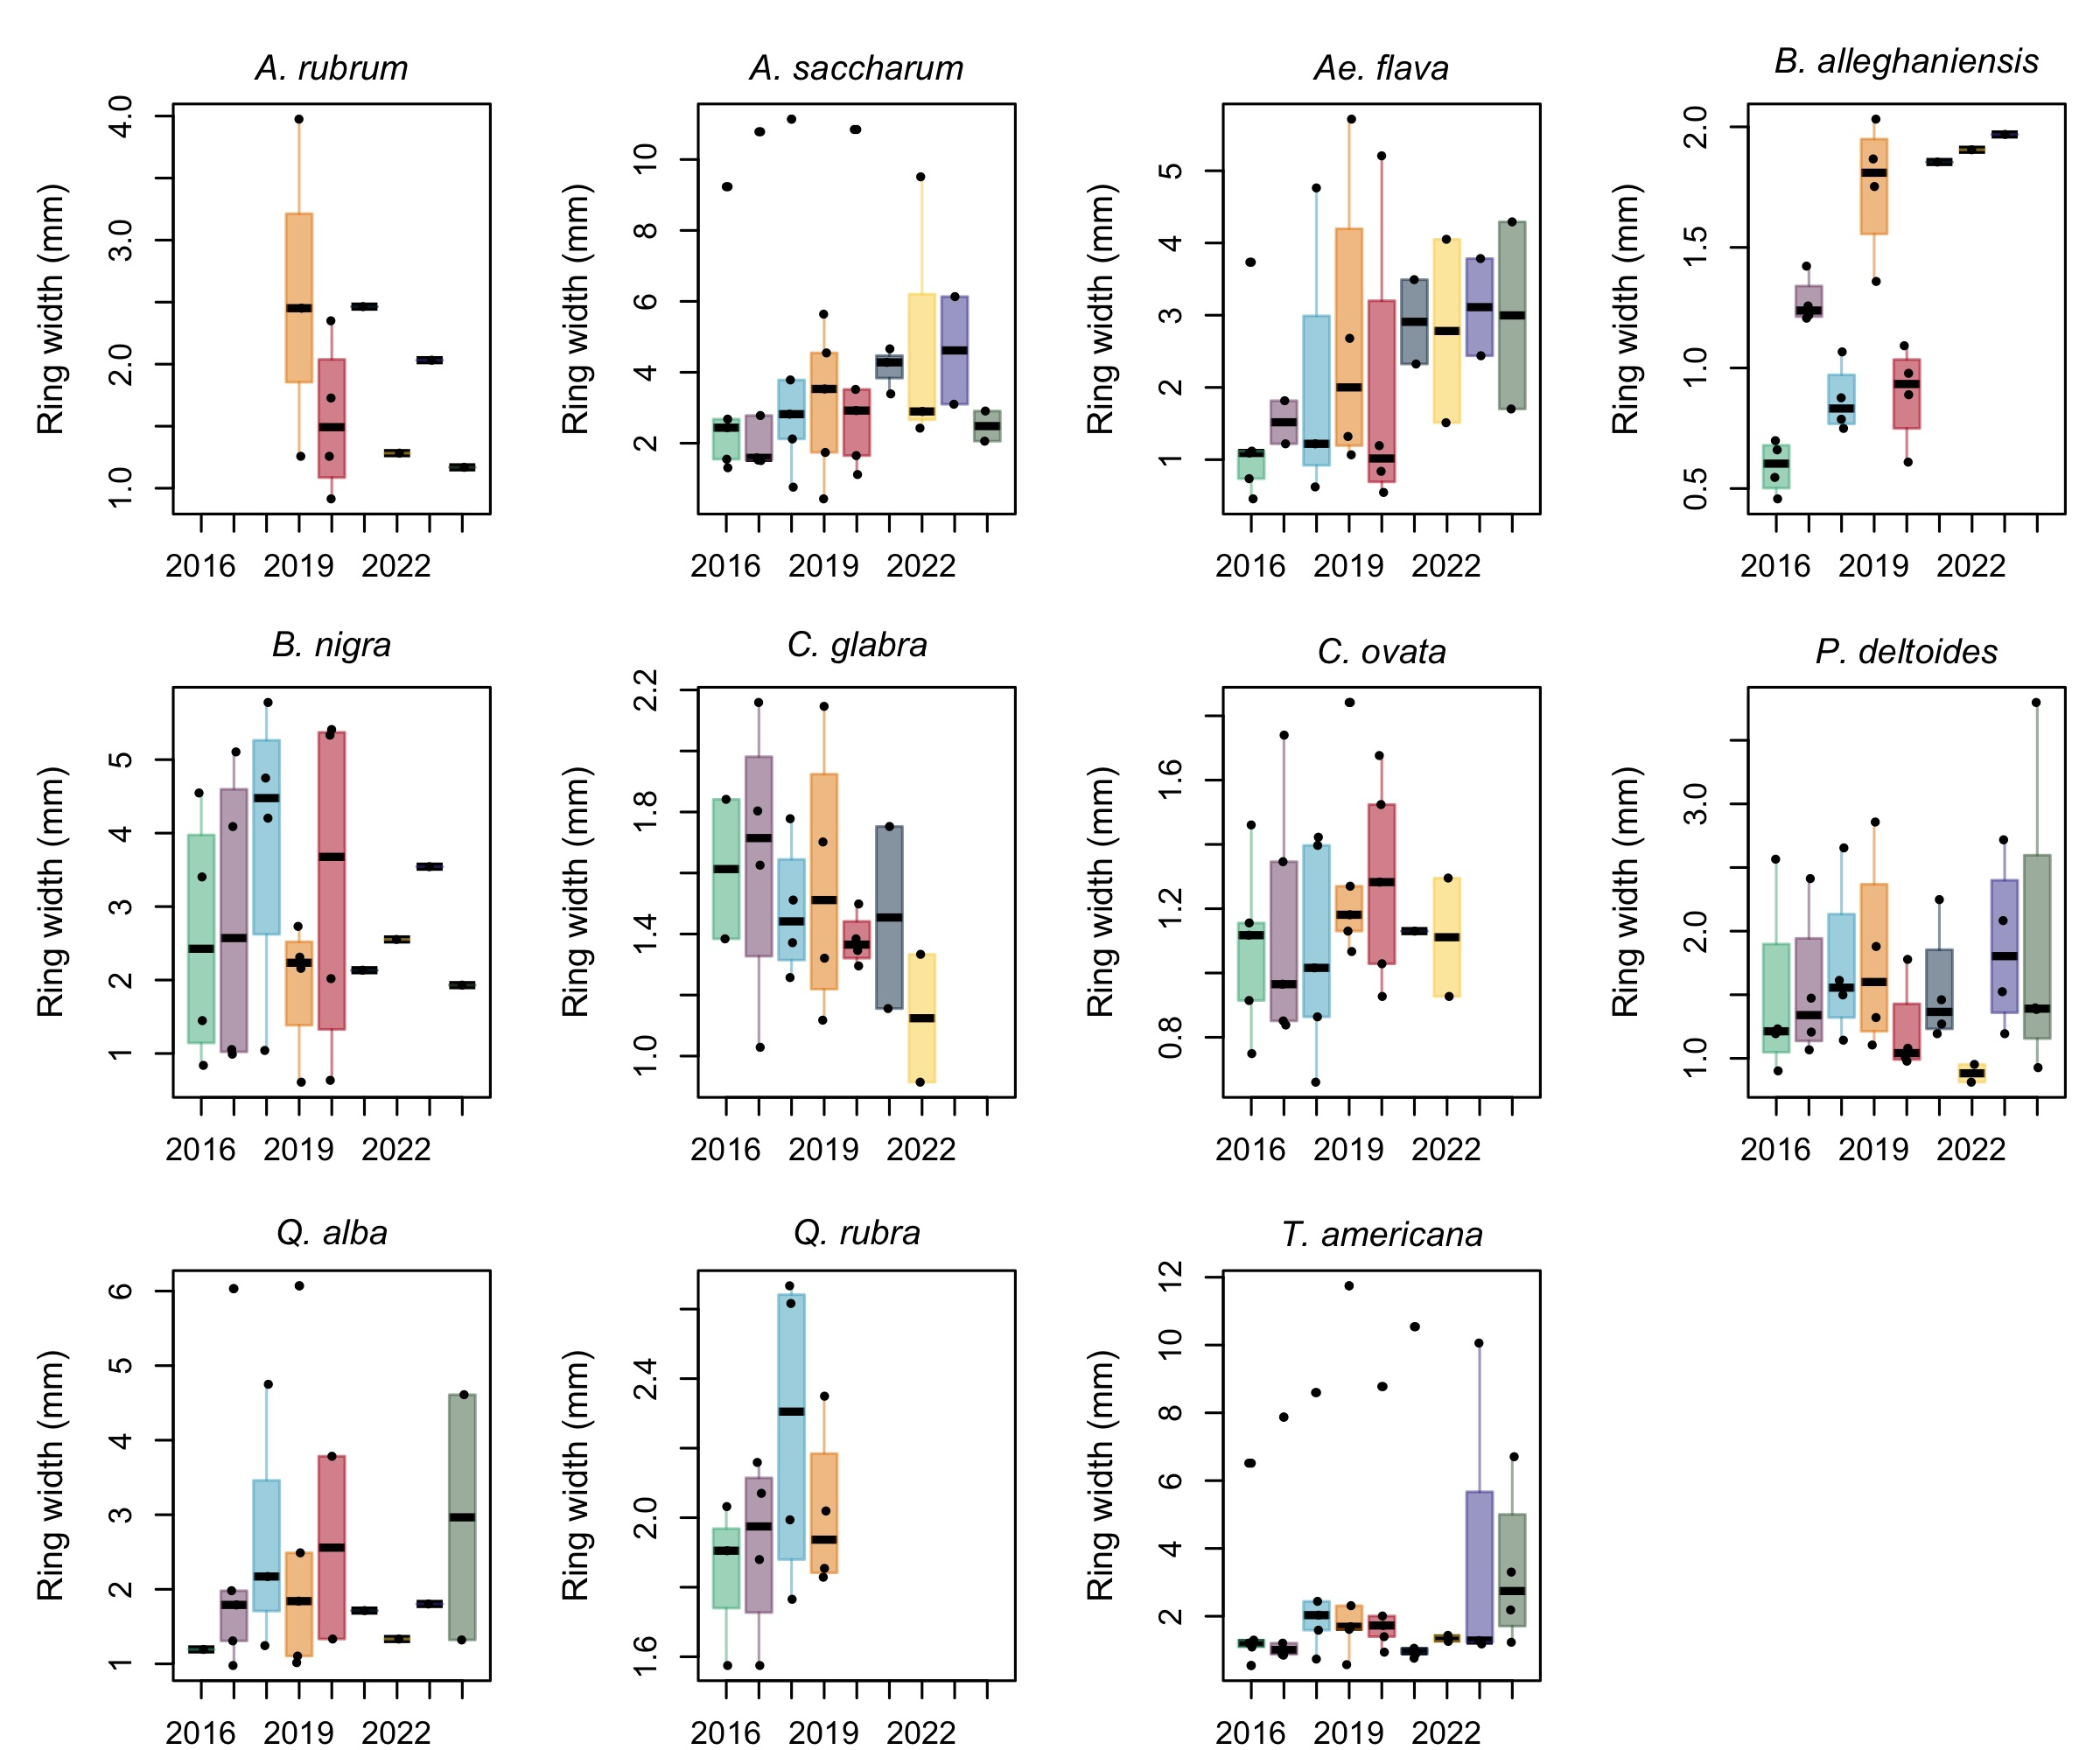
\includegraphics[width=1\textwidth]{../../analyses/figures/growthModelsMain/boxplotRingWidth.jpeg}
\caption{Boxplot representing the empirical data of our ring widths (mm) across years, facetted by species. The dots represent the raw data, the line the mean and the box the interquantile range (IQR).}
\label{fig:tsboxplot}
\end{figure}

% XY facetted by species GDD shaped by tree id
\begin{figure}[!ht]
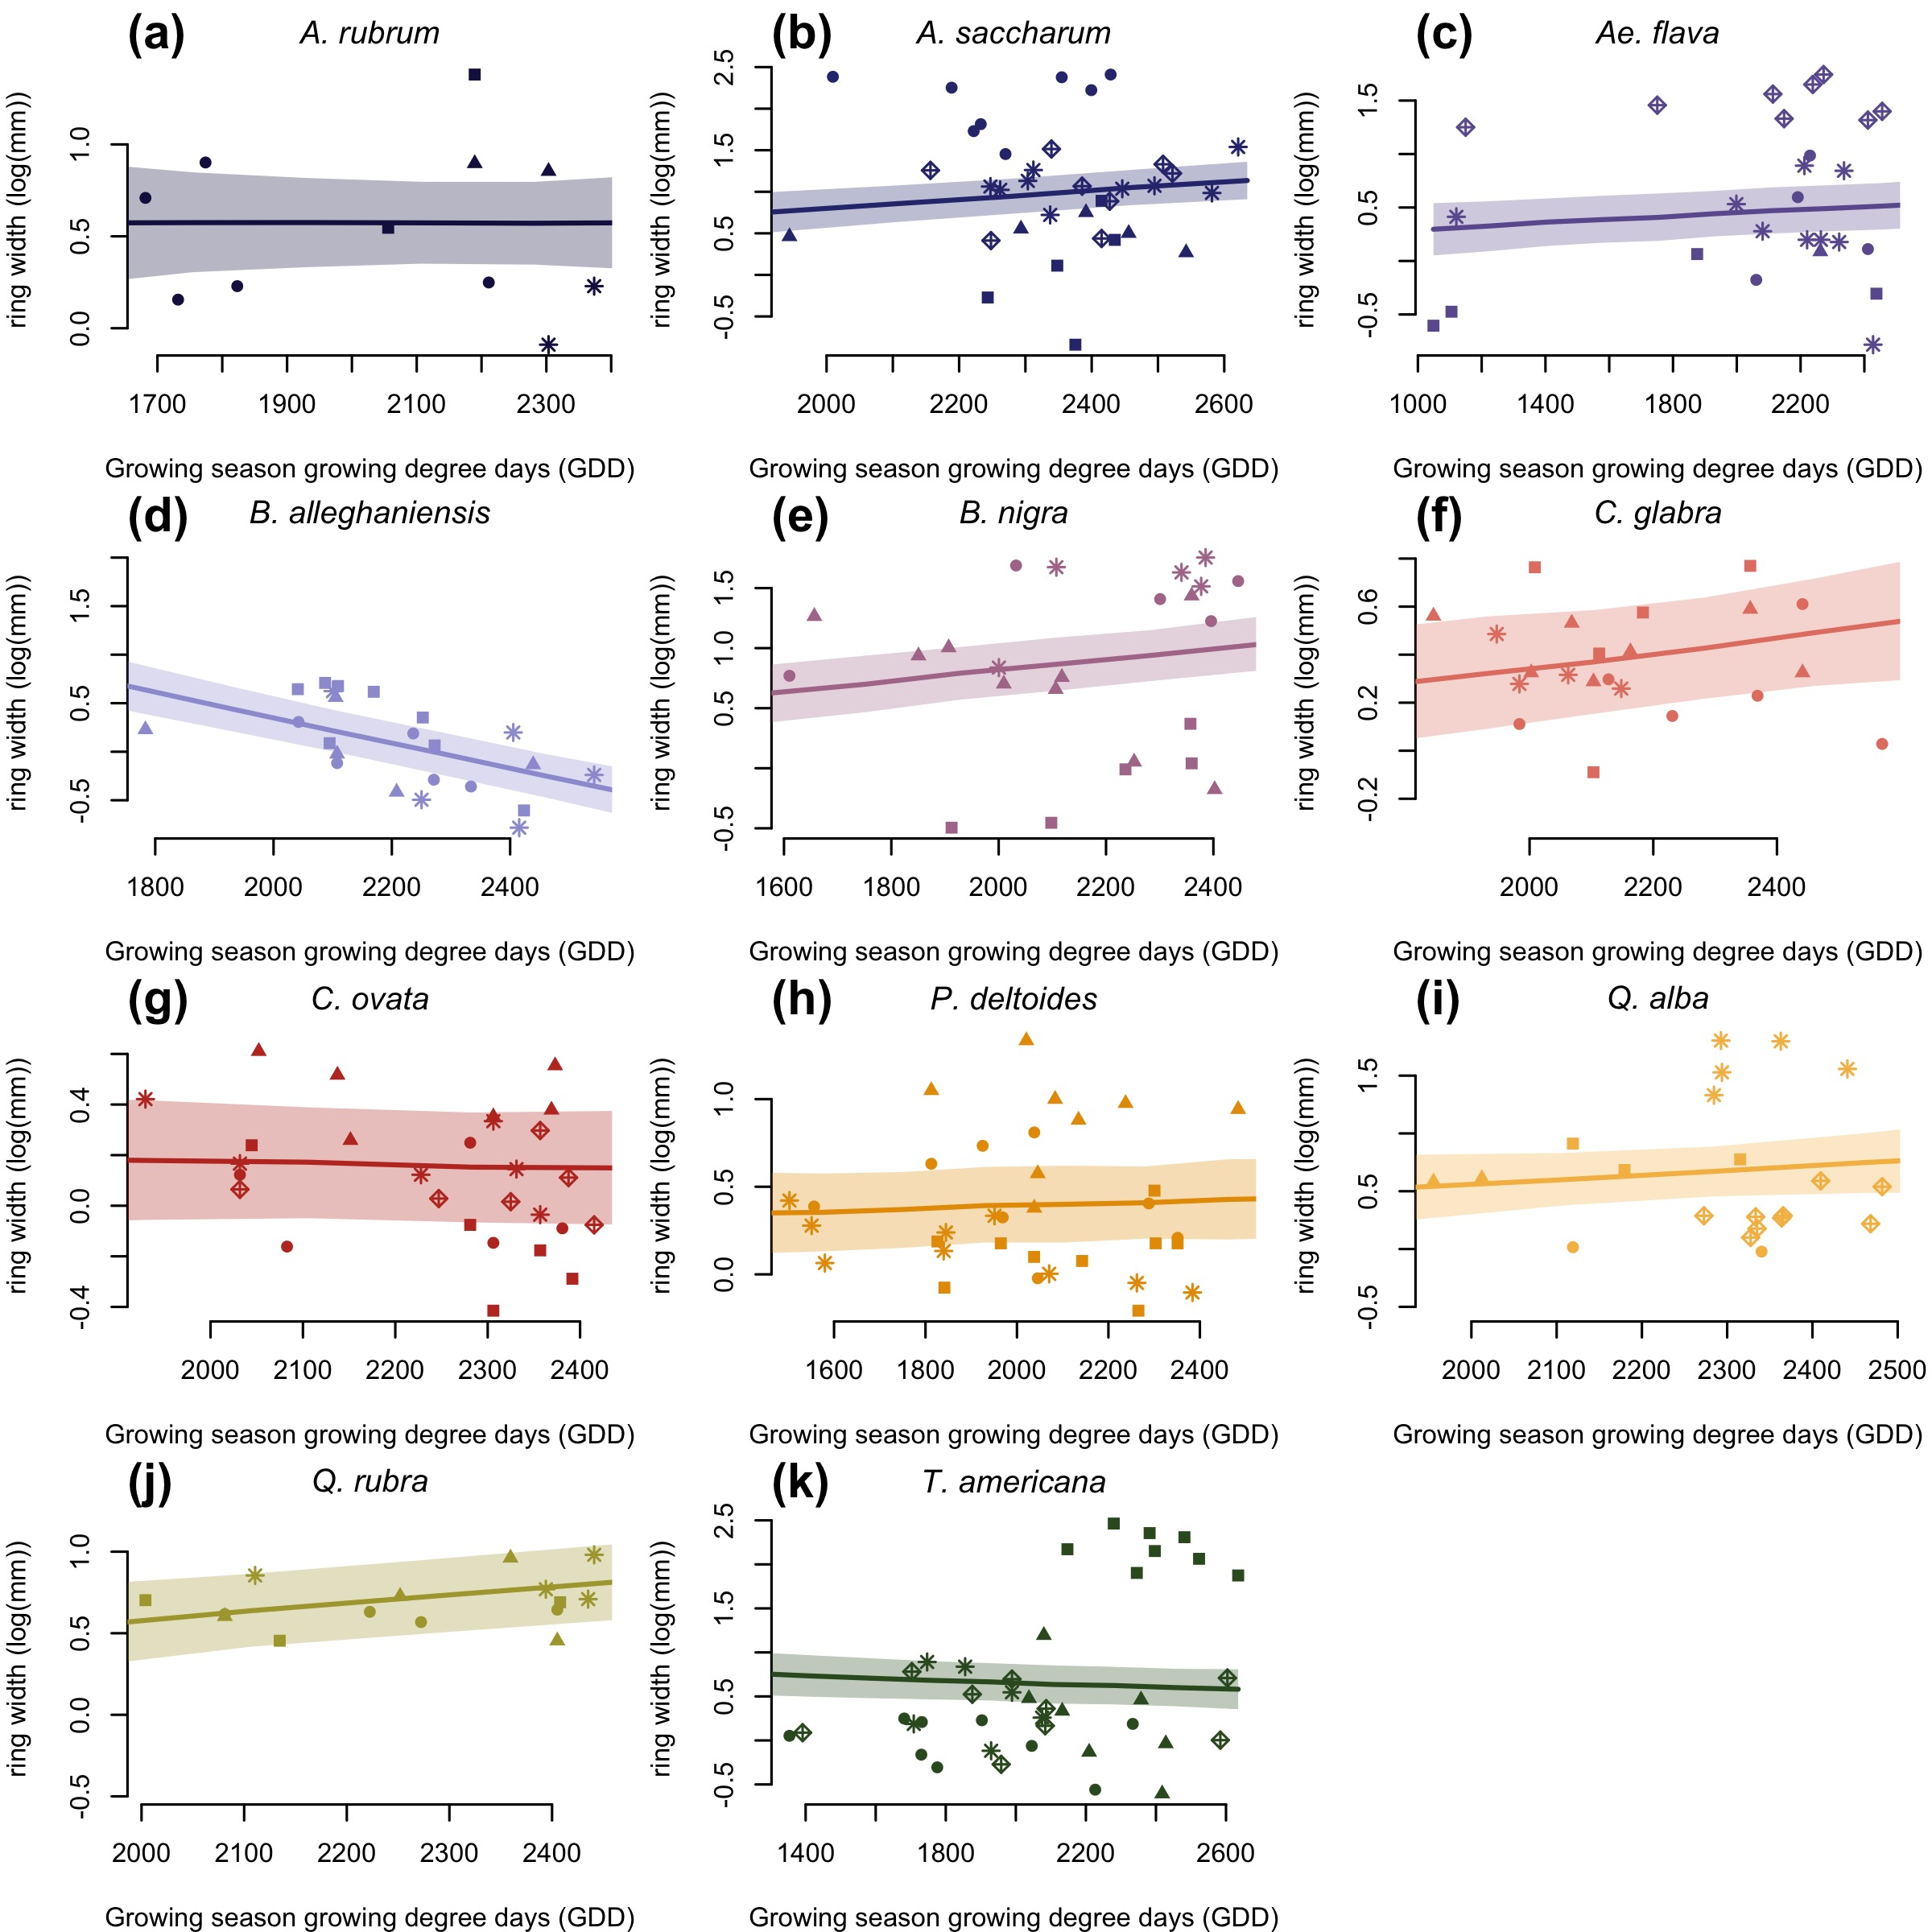
\includegraphics[width=0.8\textwidth]{../../analyses/figures/growthModelsMain/TSgrowthModelSlopesperSppFacetGDDtree.jpeg}
\caption{Ring width (log(mm)) trends in response to thermal season (GDD). The plots are the reconstructed species estimates posterior distribution with error. The lines represent the mean of the posterior distribution and the shaded area, the 50\% UI. The dots are the empirical data shaped by treeids.}
\label{fig:tsxyGDDtree}
\end{figure}

% XY facetted by species GSL shaped by tree id
\begin{figure}[!ht]
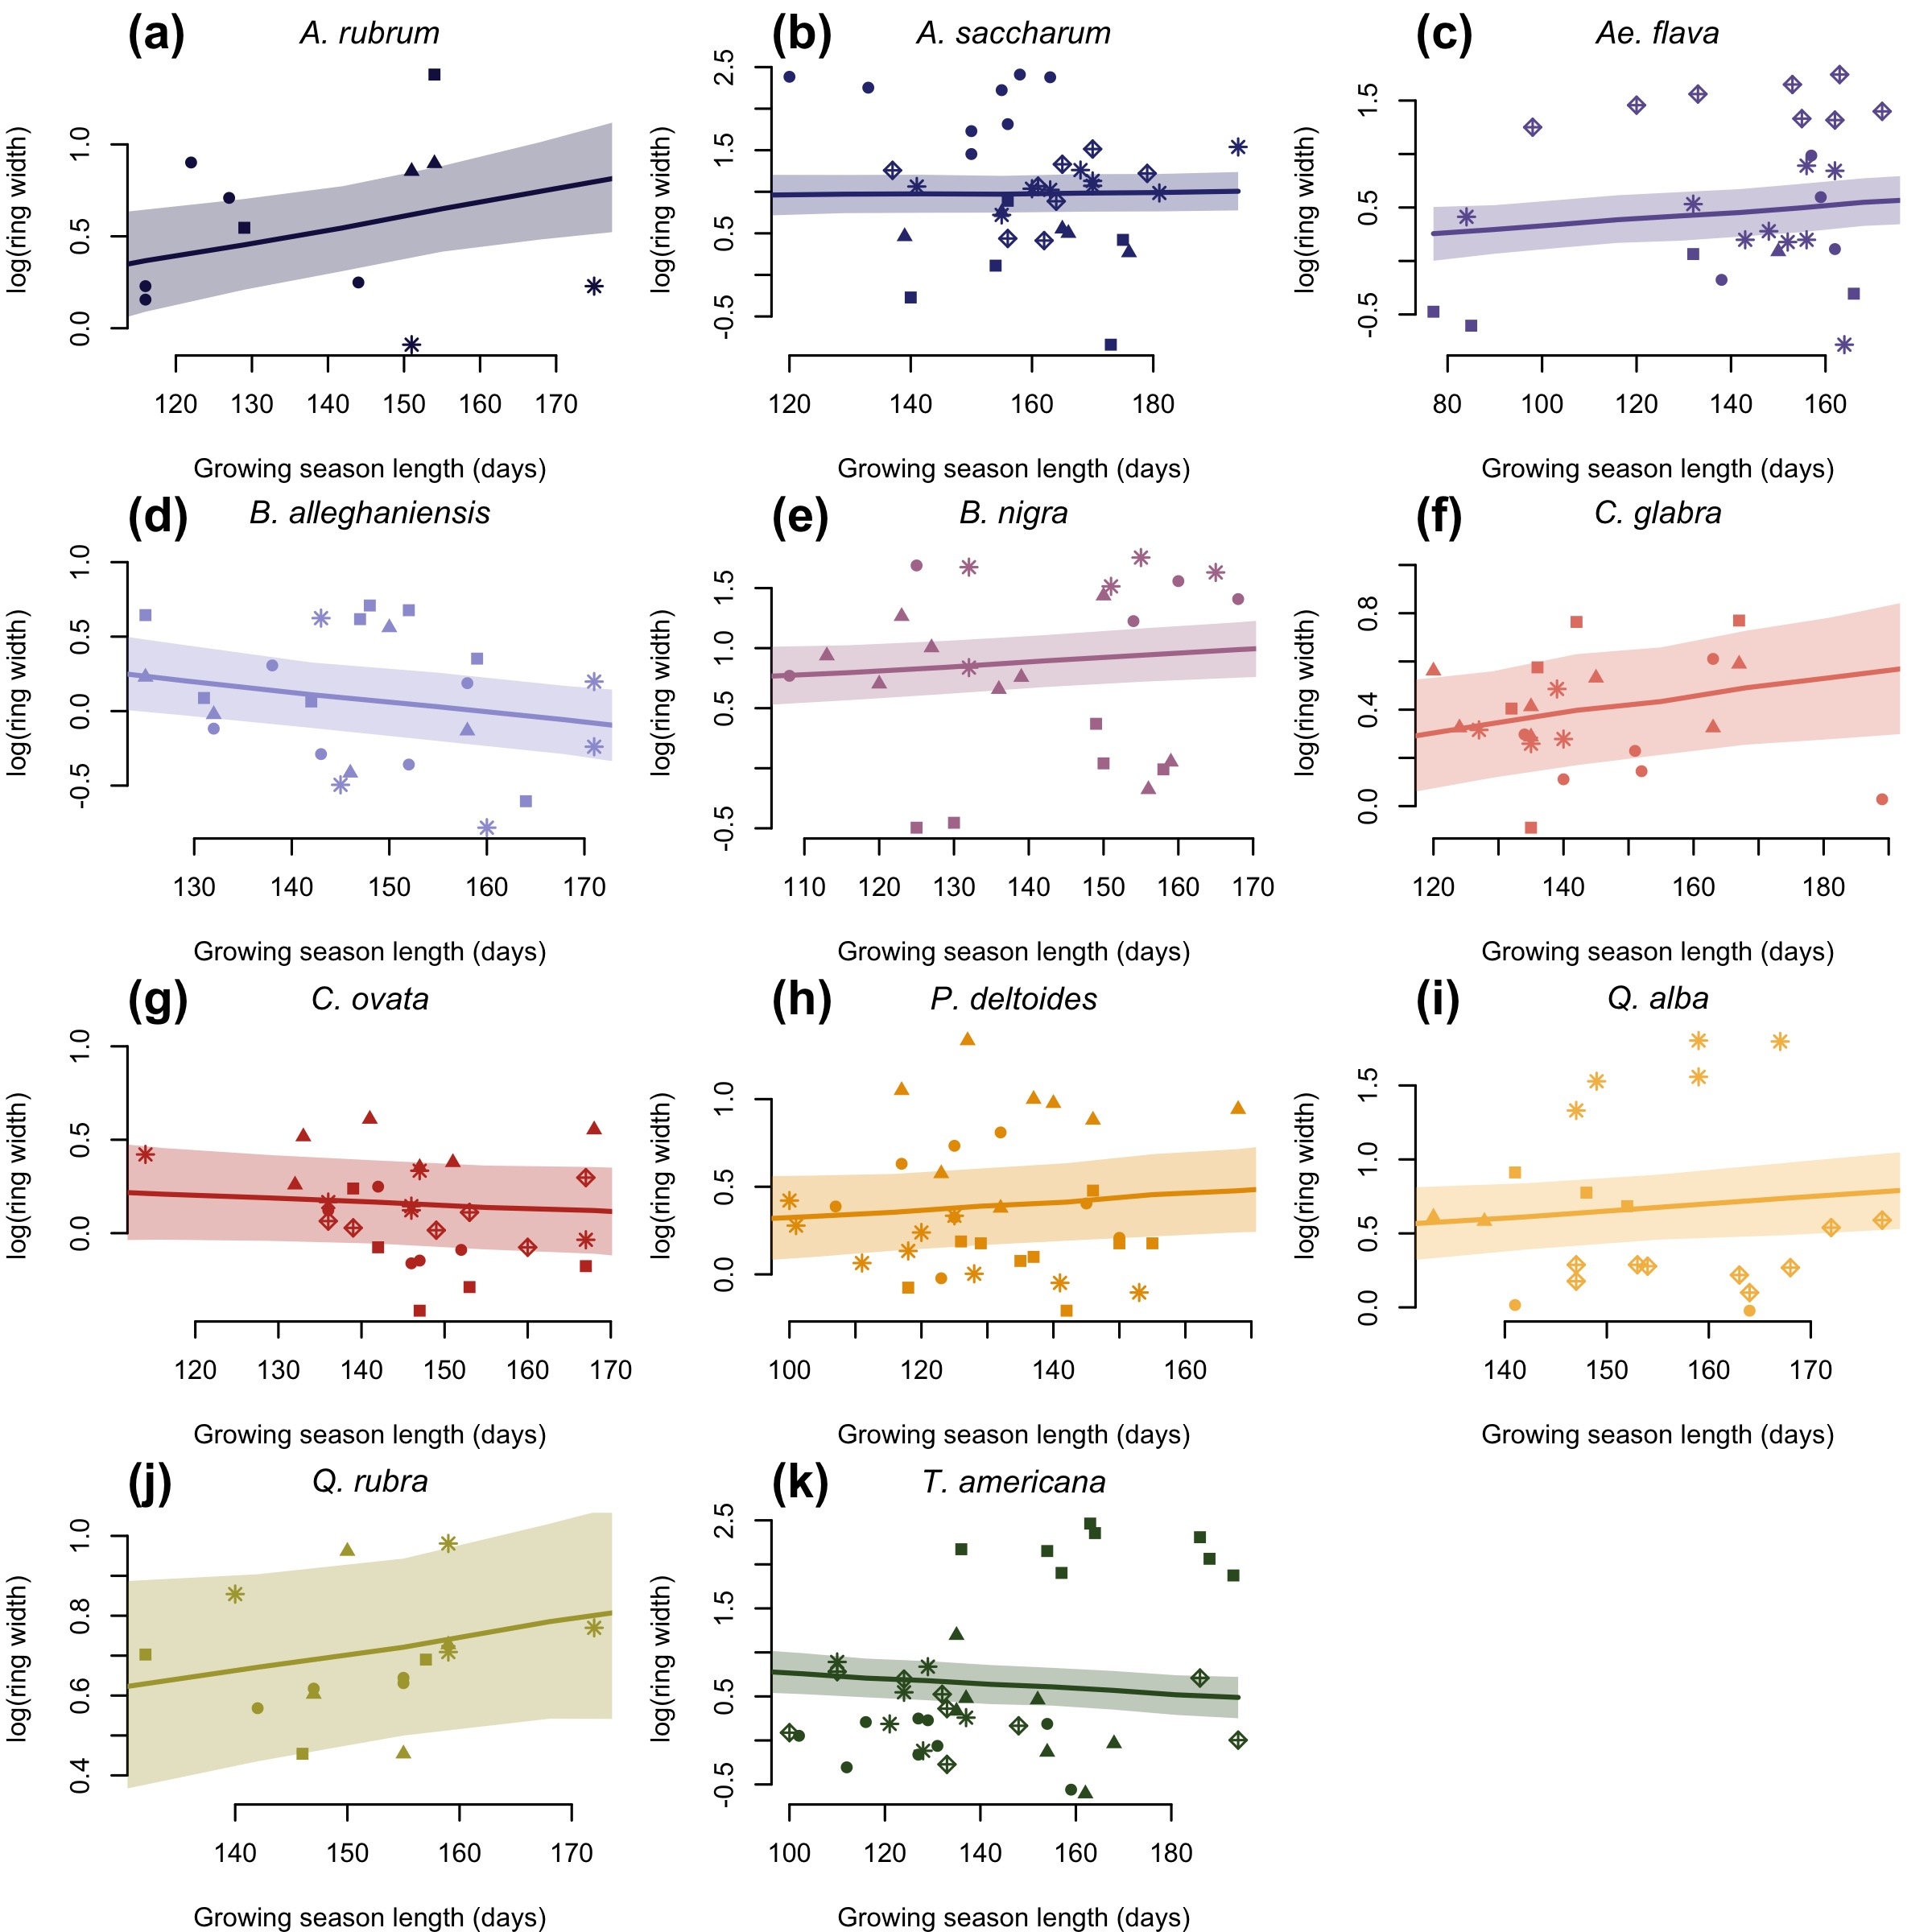
\includegraphics[width=0.8\textwidth]{../../analyses/figures/growthModelsMain/TSgrowthModelSlopesperSppFacetGSLtree.jpeg}
\caption{Ring width trends (log(mm)) in response to calendar season (GSL). The plots are the reconstructed species estimates posterior distribution with error. The lines represent the mean of the posterior distribution and the shaded area, the 50\% UI. The dots are the empirical data shaped by treeids.}
\label{fig:tsxyGSLtree}
\end{figure}

% XY facetted by species GDD shaped by year
\begin{figure}[!ht]
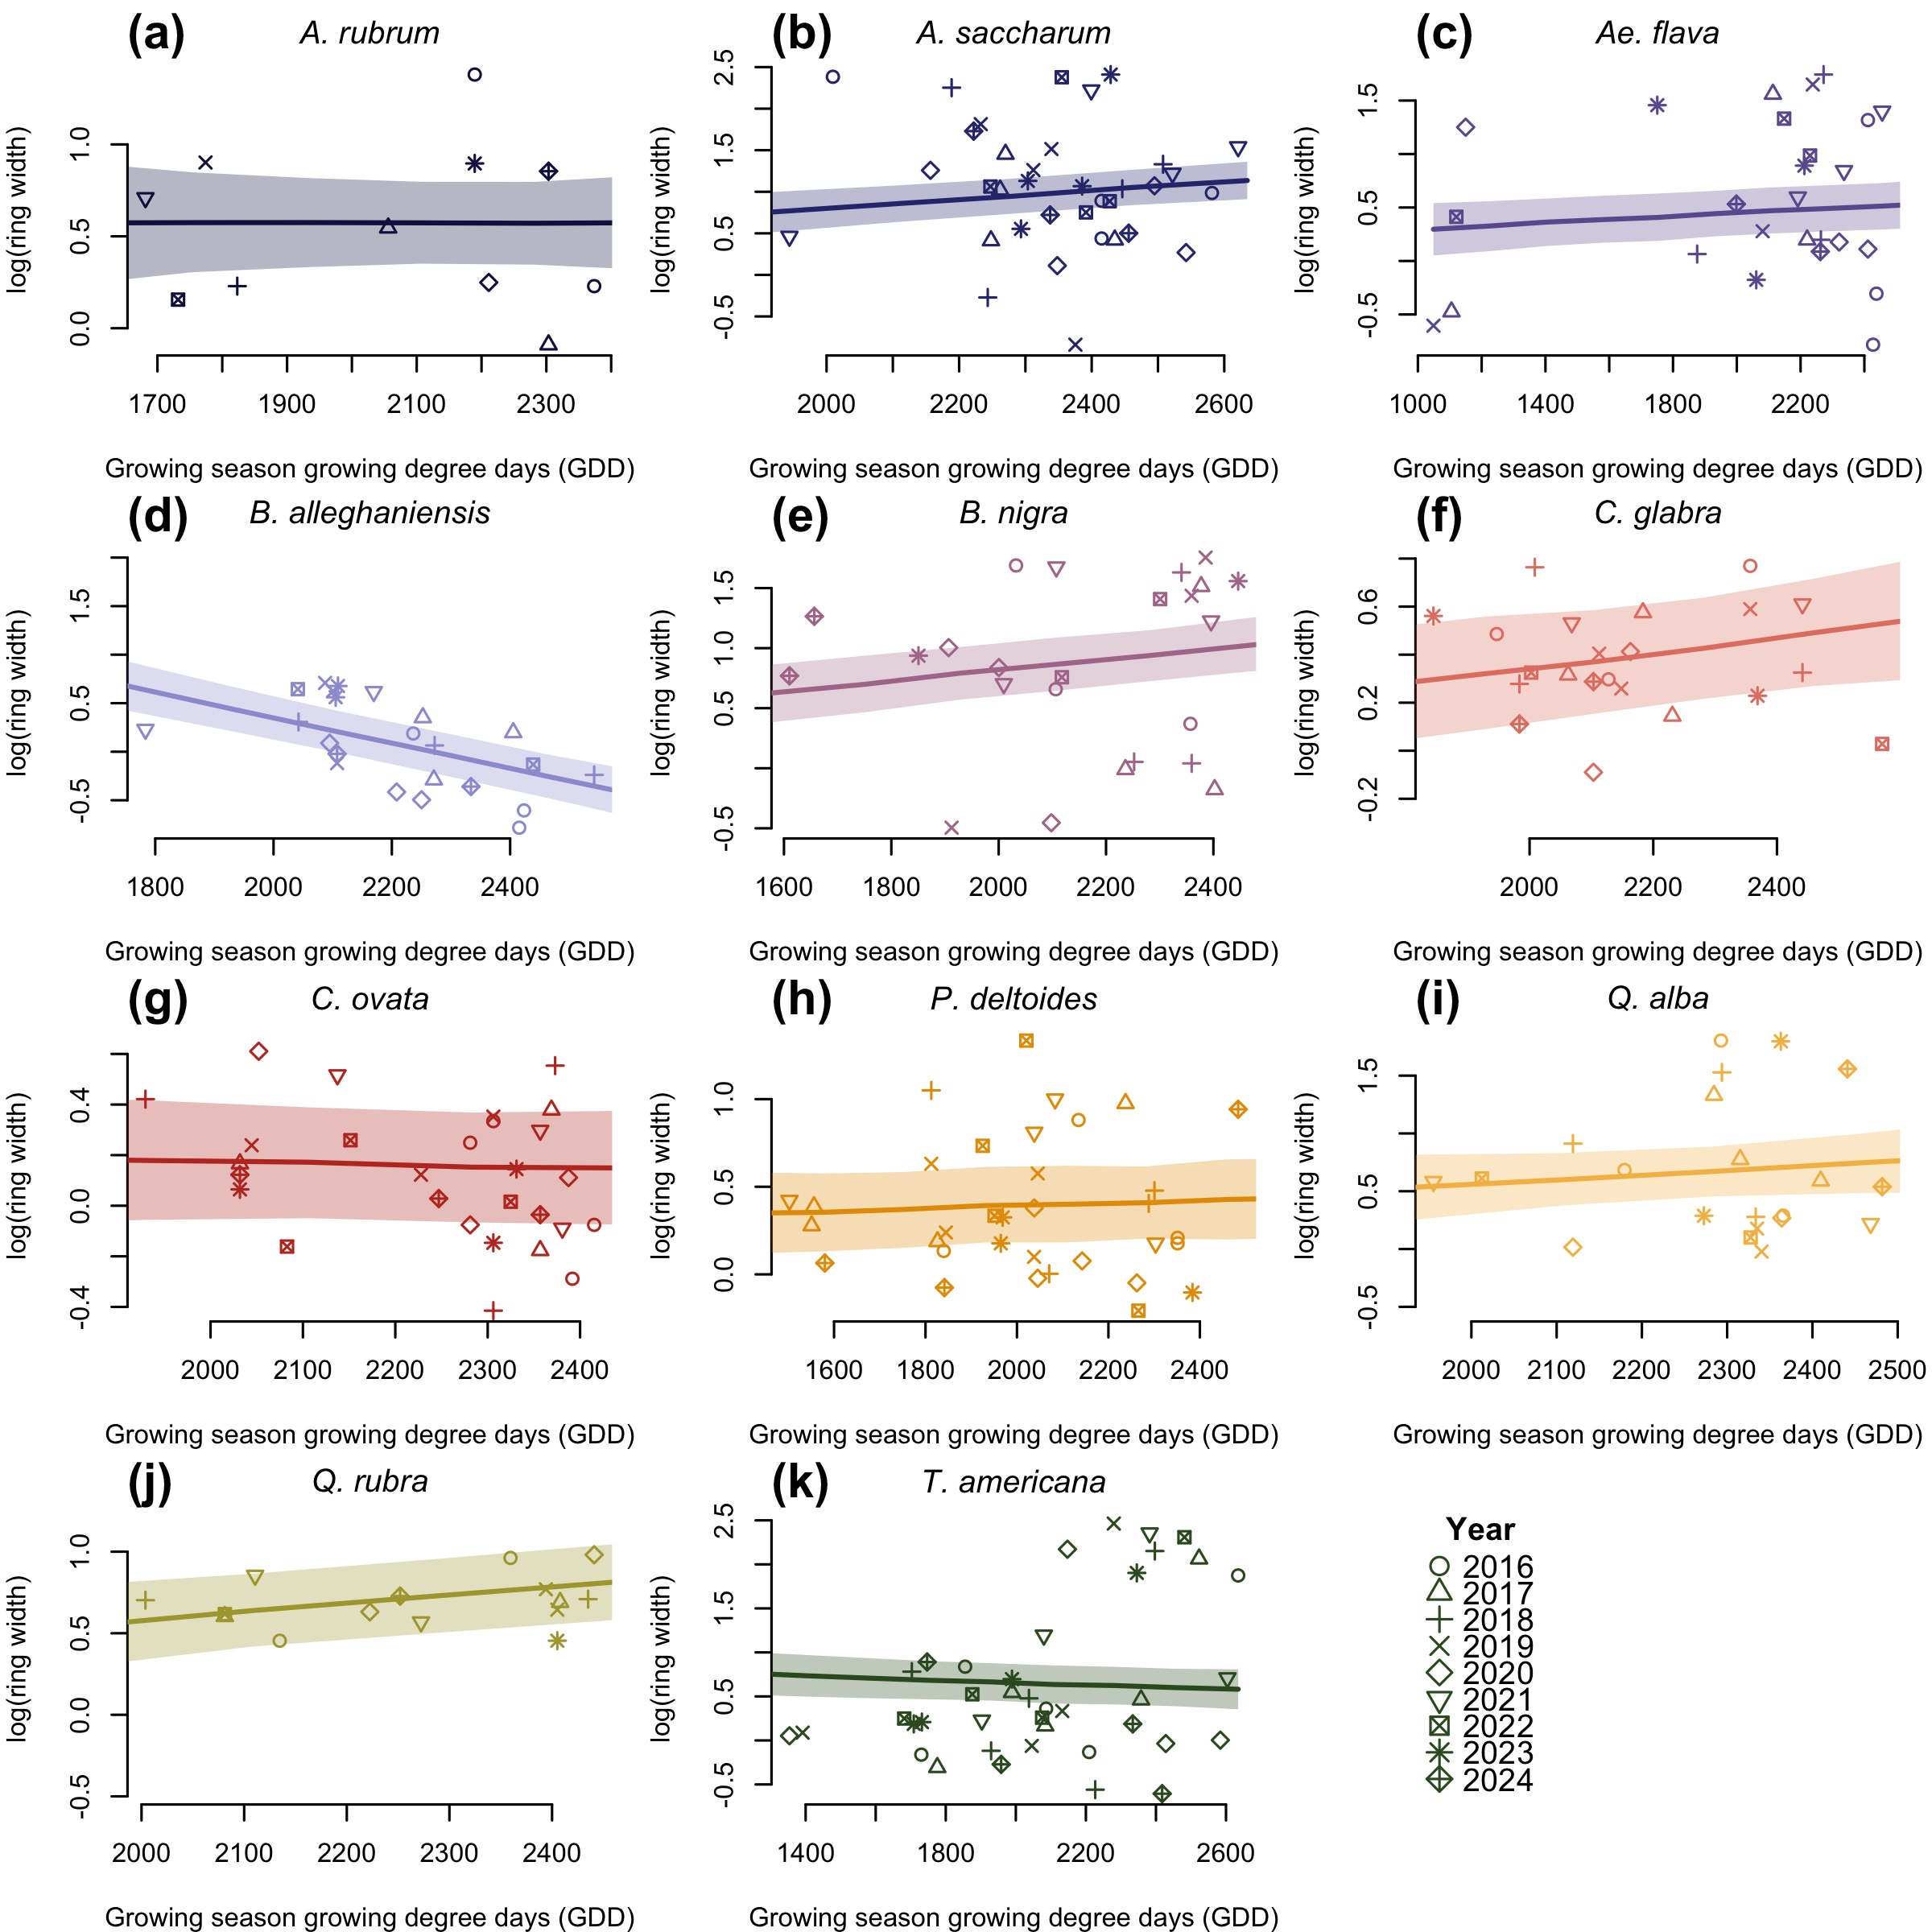
\includegraphics[width=0.8\textwidth]{../../analyses/figures/growthModelsMain/TSgrowthModelSlopesperSppFacetGDDyr.jpeg}
\caption{Ring width trends (log(mm)) in response to thermal season (GDD). The plots are the reconstructed species estimates posterior distribution with error. The lines represent the mean of the posterior distribution and the shaded area, the 50\% UI. The dots are the empirical data shaped by year.}
\label{fig:tsxyGDDyr}
\end{figure}

% XY facetted by species GSL shaped by year
\begin{figure}[!ht]
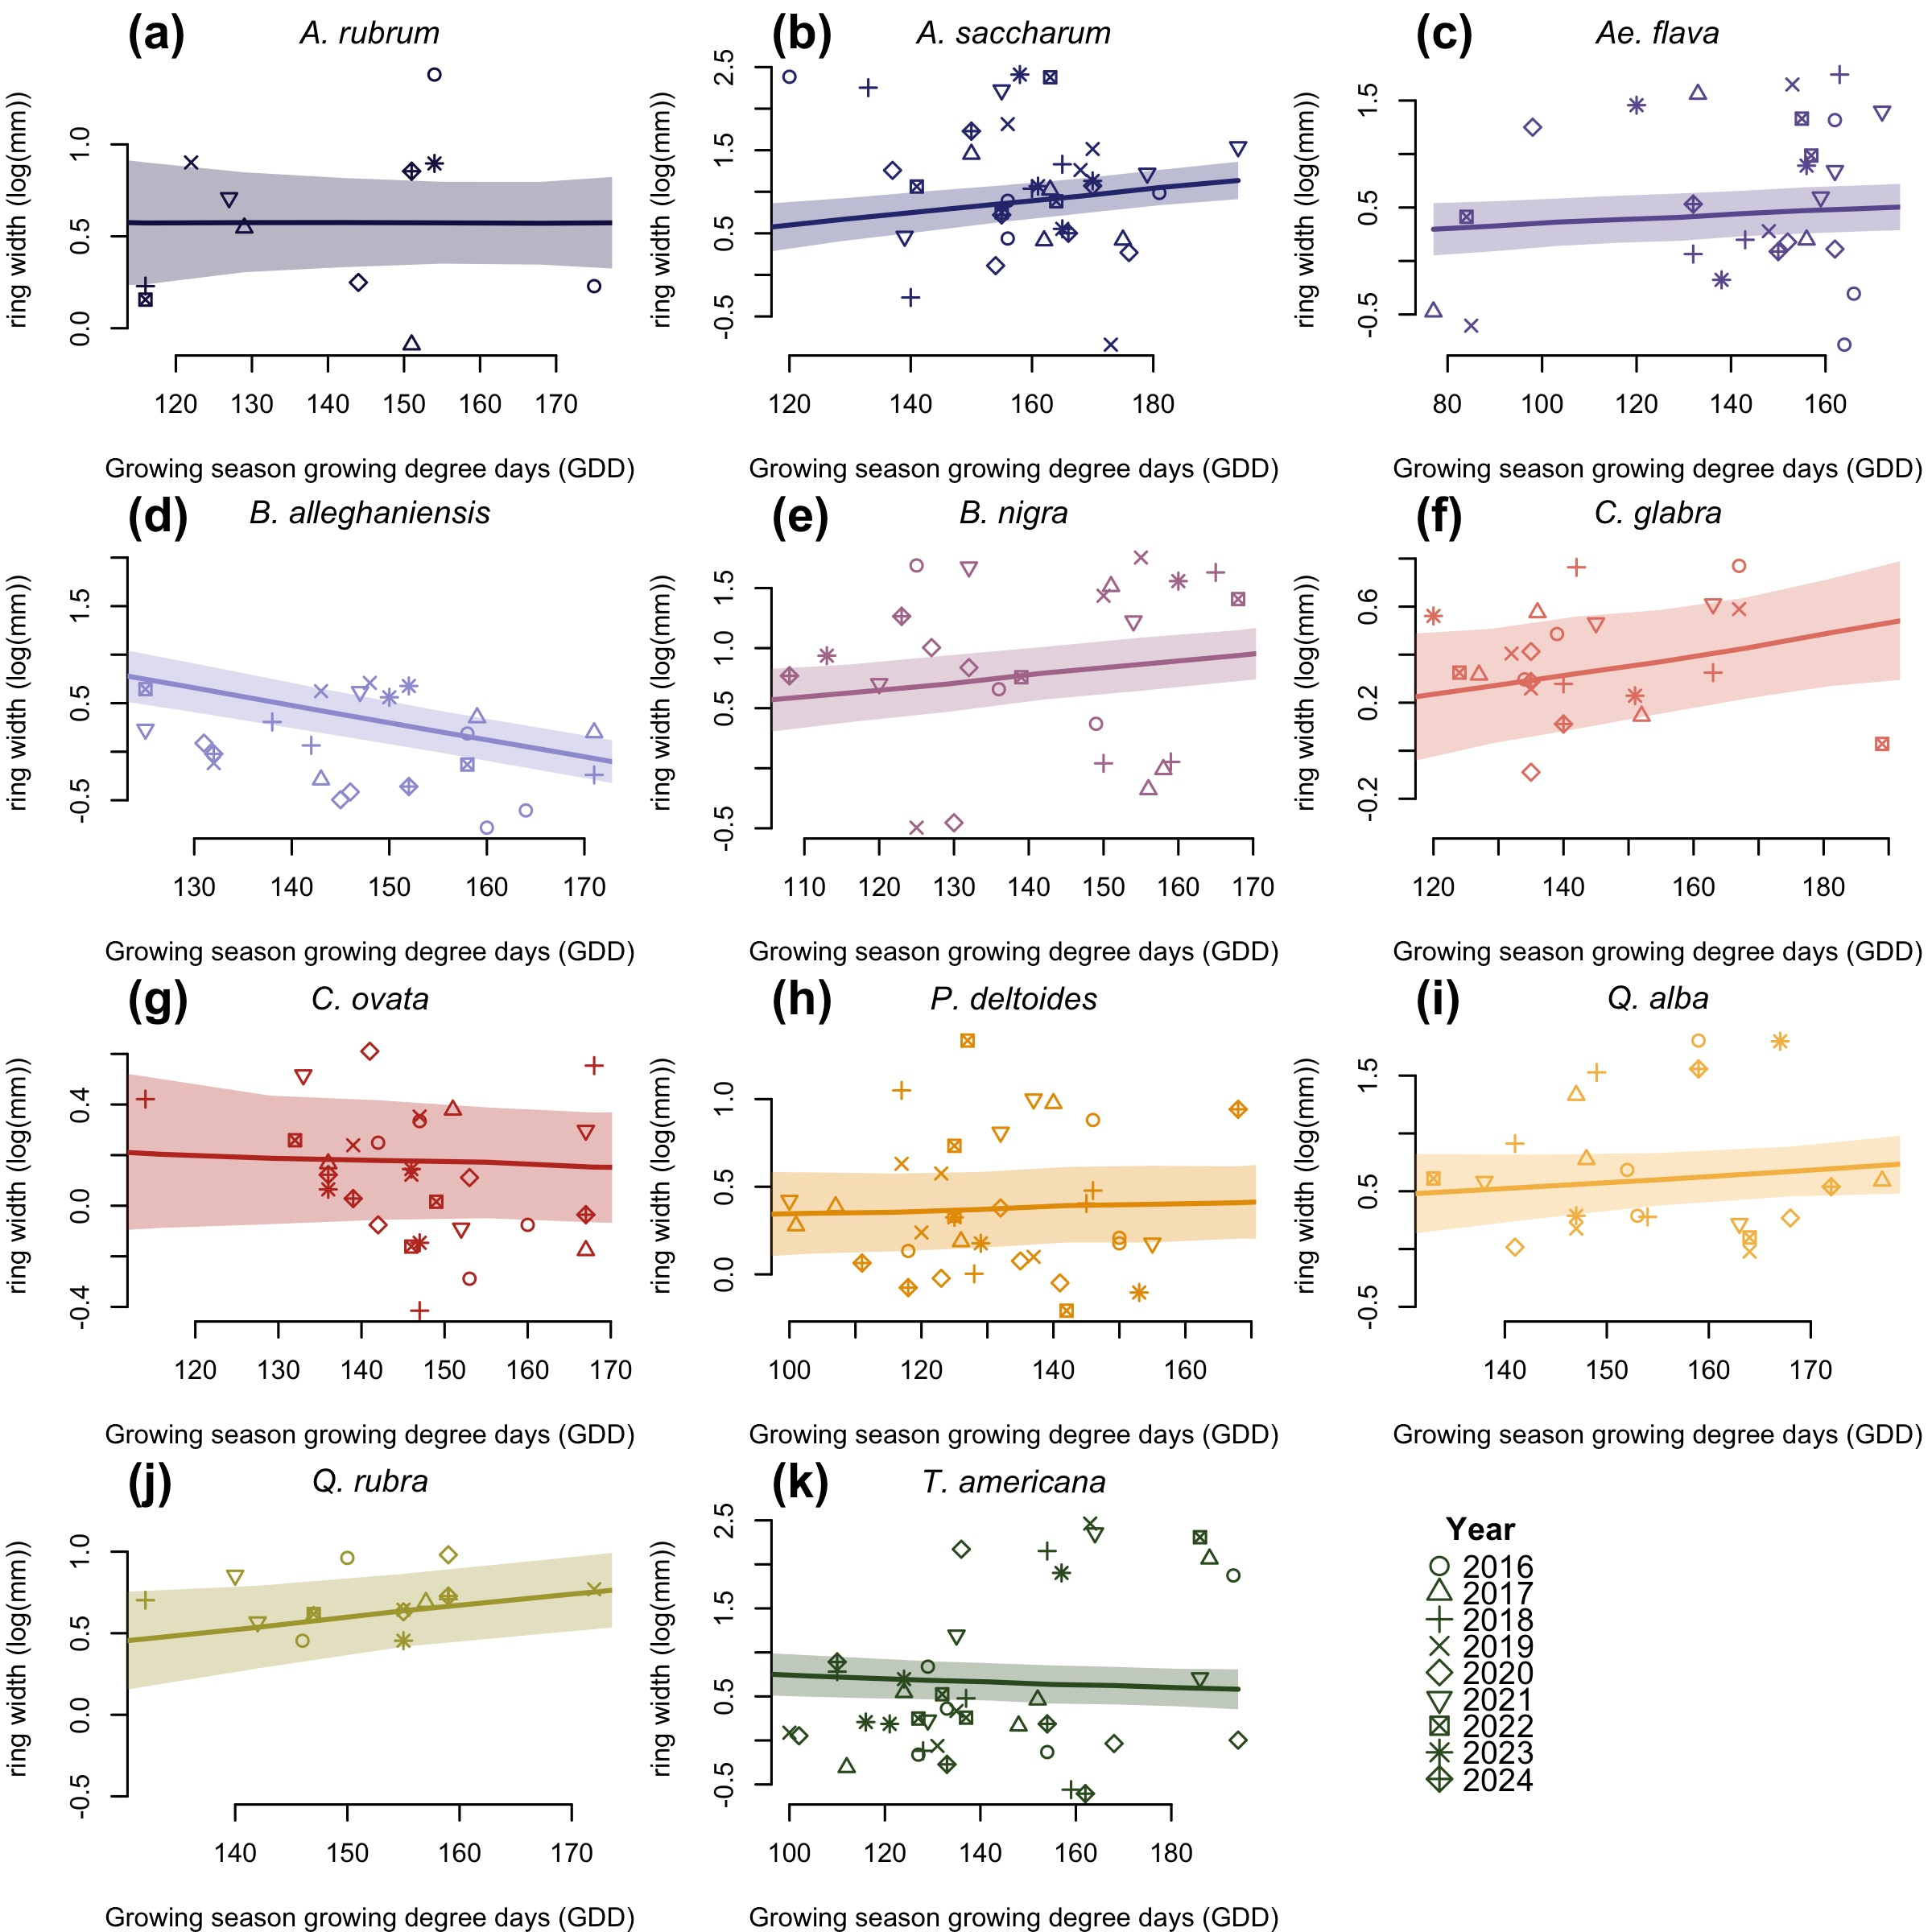
\includegraphics[width=0.8\textwidth]{../../analyses/figures/growthModelsMain/TSgrowthModelSlopesperSppFacetGSLyr.jpeg}
\caption{Ring width trends (log(mm)) in response to calendar season (GSL). The plots are the reconstructed species estimates posterior distribution with error. The lines represent the mean of the posterior distribution and the shaded area, the 50\% UI. The dots are the empirical data shaped by year.}
\label{fig:tsxyGSLyr}
\end{figure}

% Figure mu atreeid full
\begin{figure}[!ht]
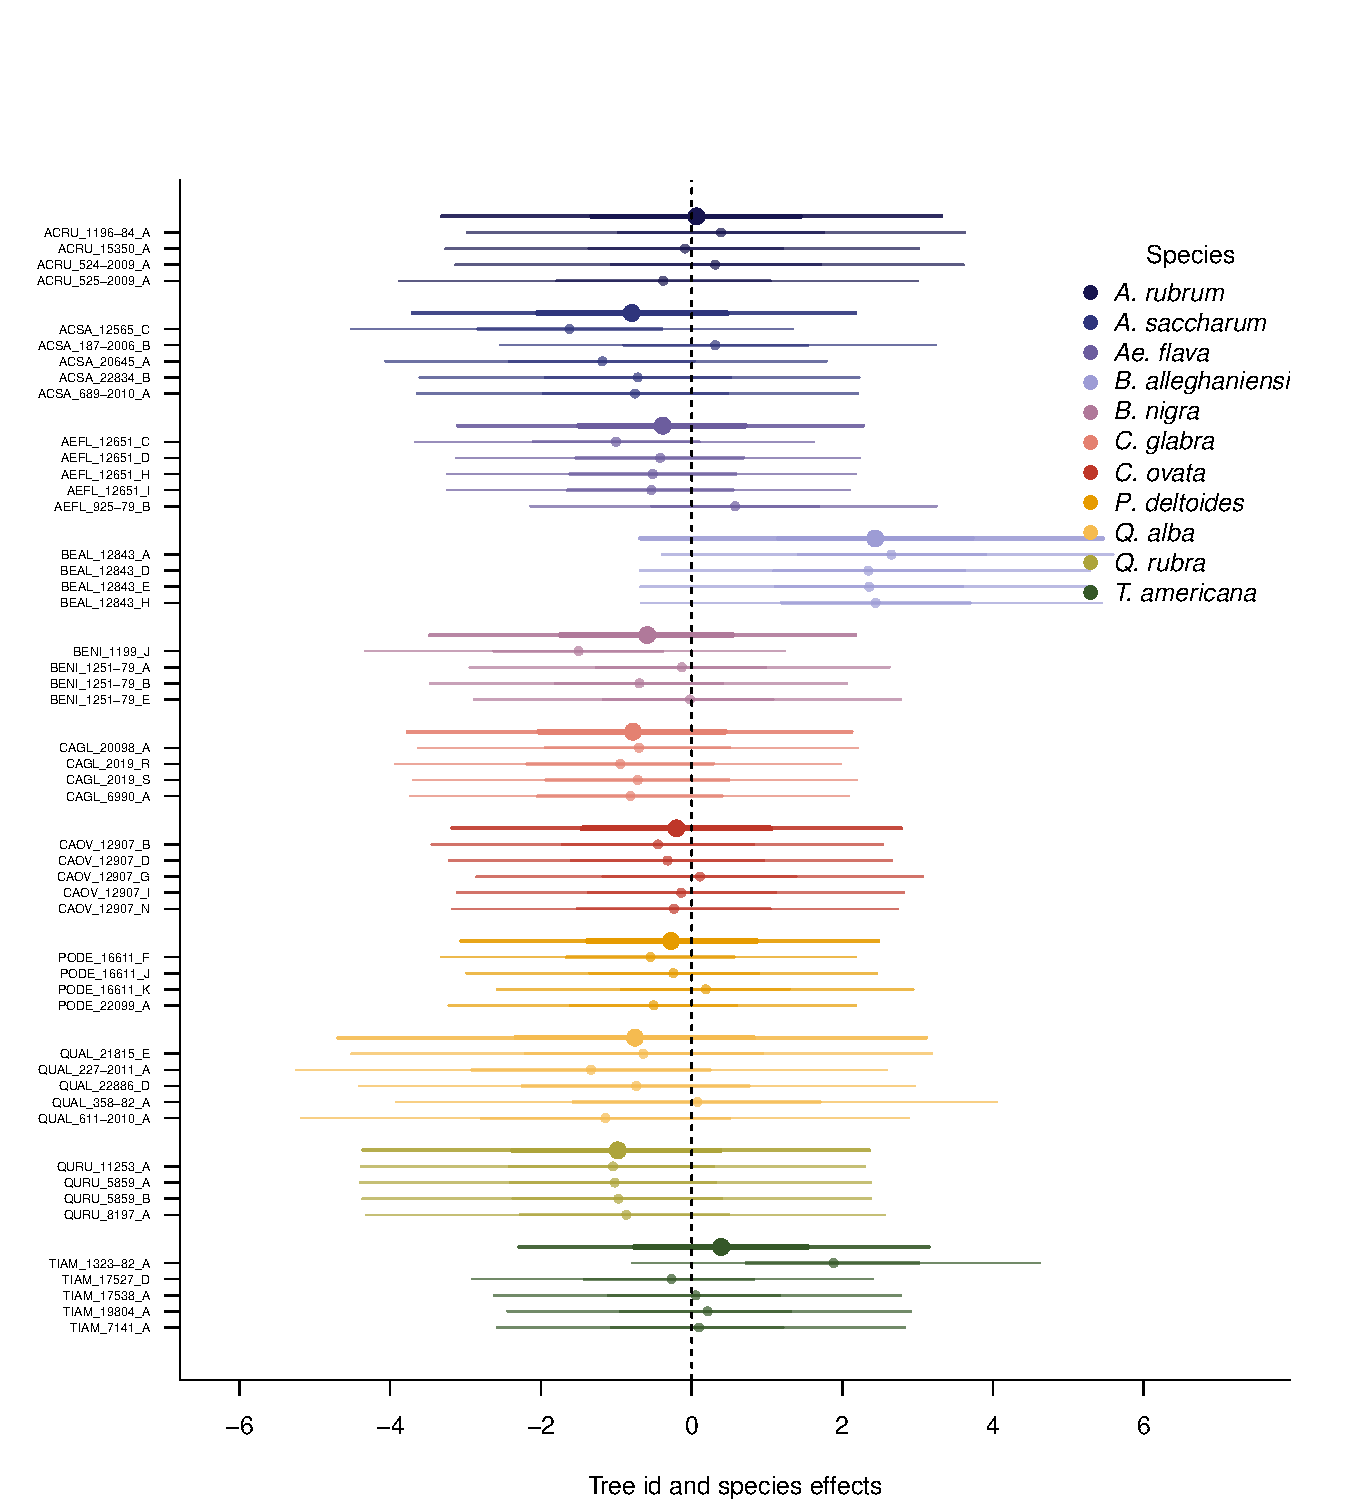
\includegraphics[width=0.8\textwidth]{../../analyses/figures/growthModelsMain/TSmeanPlotGrowthGDD_treeidBYspp.pdf}
\caption{Ring width (log(mm)) deviations from the grand mean for each grouping factor of the GDD model. The different tree id values represent the combined intercepts of tree id, species and averaged year intercepts. The larger dots and lines represent the species intercepts which are the species level estimates averaged across all of their tree ids. The dots are the mean of the posterior distribution and the thick and thin lines, the 50 and 90\% UI.}
\label{fig:tsmuplotatreeid}
\end{figure}

% Full vs restricted data comparison for Coringtreespotters
\begin{figure}[!ht]

\includegraphics[width=1\textwidth]{/Users/christophe_rouleau-desrochers/github/coringtreespotters/analyses/figures/growthModelsMain/FullVSRestricted.pdf}
\caption{Full vs, most restricted rows of data for the model with start of season (SOS; a) and end of season (EOS; b) as the predictor. Each panel represent the different parameters used to fit the models. $\alpha_{species}$ and $\alpha_{year}$ represent the ring width (log(mm)) for species and year, respectively. $\beta_{species}$ represent the change in ring width (log(mm)) per scaled predictor for each species (see `Data analyses' section in Methods for more details on predictor scaling).} 
\label{fig:tsSOSEOScomparison}
\end{figure}

% Budburst vs leafout for CoringTreespotters
\begin{figure}[!ht]

\includegraphics[width=0.8\textwidth]{/Users/christophe_rouleau-desrochers/github/coringtreespotters/analyses/figures/growthModelsMain/budburstVSLeafout/DporousVSRporous.pdf}
\caption{Parameter estimates when calculating the GDD (a), GSL (b) from leafout vs budburst, to leaf coloring. (c) shows the model estimates when taking leafout vs budburst as the SOS (see `Data analyses' section in Methods for more details).}
\label{fig:buburstVSleafoutTS}
\end{figure}

% Z-scored slope results
\begin{figure}[!ht]
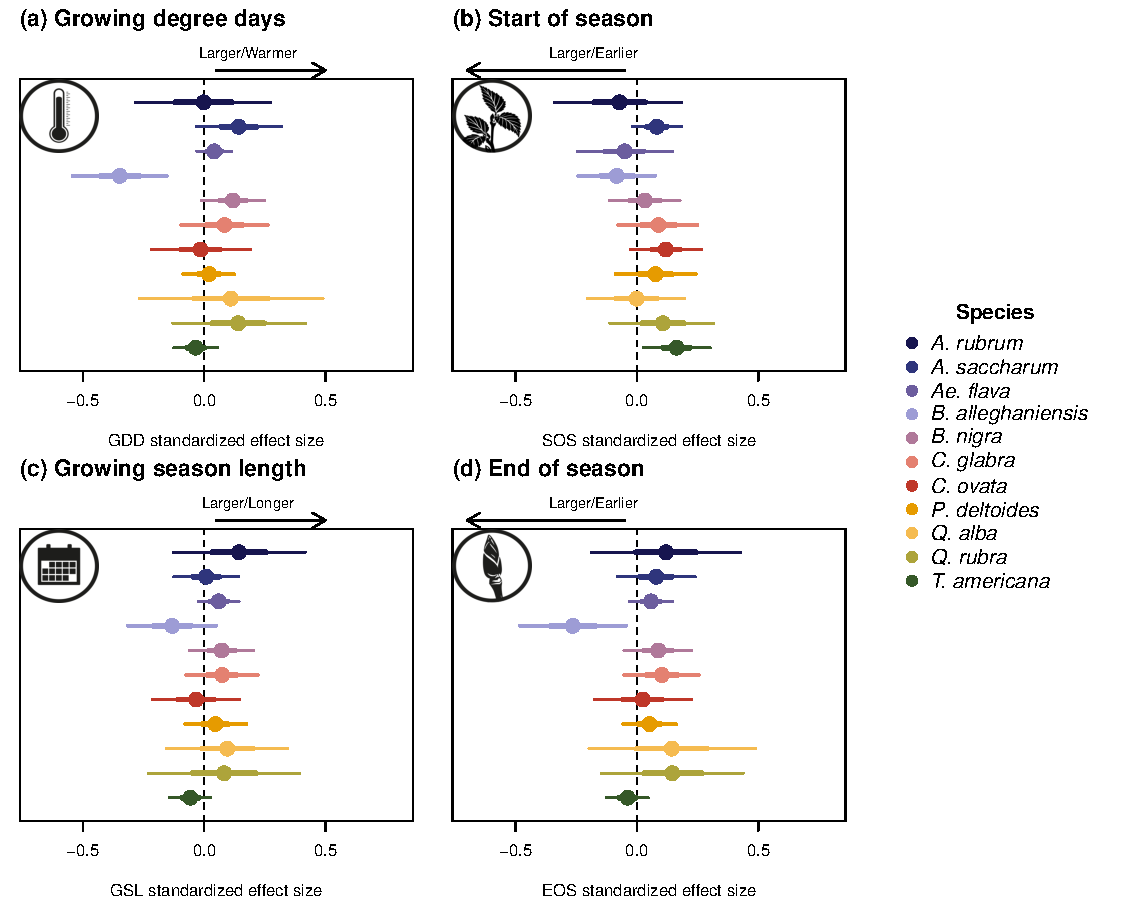
\includegraphics[width=0.8\textwidth]{../../analyses/figures/growthModelsMain/zscored/muALLbsppZ.pdf}
\caption{Effect size of each predictors across our eleven species. We depict ring width (log(mm)) change per scaled ($z$-scored; see `Data analyses' section in Methods for more details) predictor for each species. We report estimates as mean and 90\% uncertainty intervals (in square brackets) across our four different predictors (GDD: growing degree days, GSL: growing season length, SOS: start of season and EOS: end of season).}
\label{fig:bsppZscored}
\end{figure}

% Carry over of SOS on EOS
\begin{figure}[!ht]
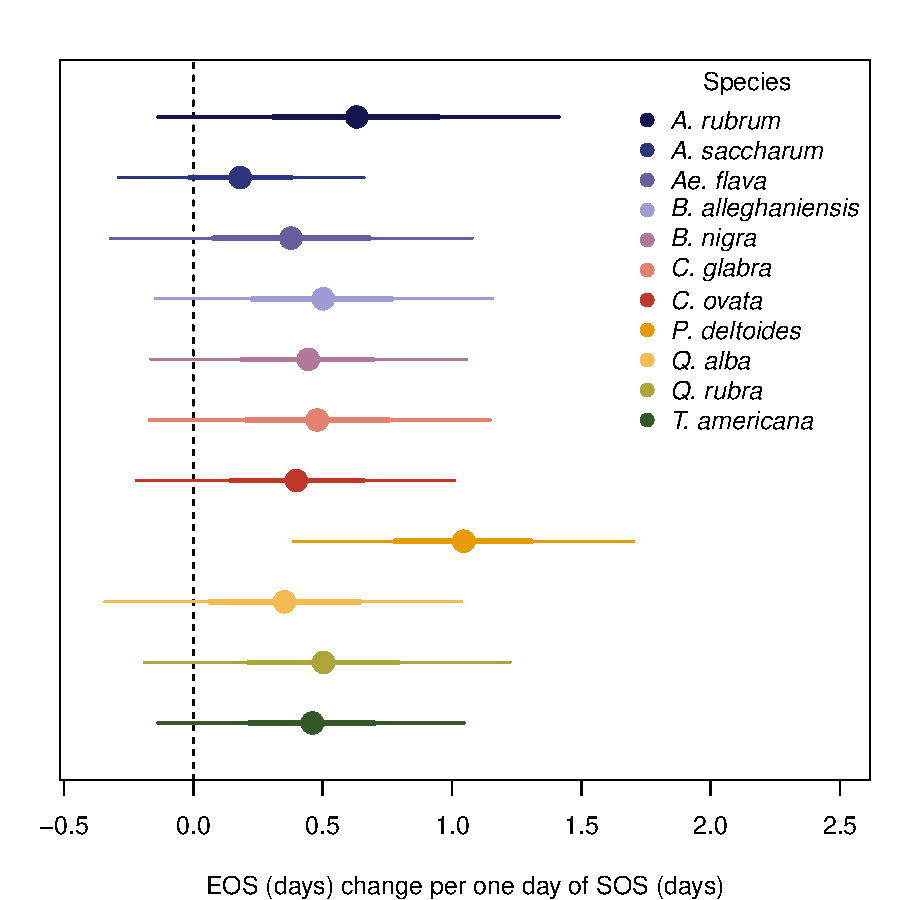
\includegraphics[width=0.8\textwidth]{../../analyses/figures/SOSonEOS/bsppSOSonEOS.pdf}
\caption{Effect of the start of season (SOS) on the end of season (EOS) across our eleven species. We report these slope estimates as mean and 90\% uncertainty intervals.}
\label{fig:SOSonEOS}
\end{figure}




\end{document}
